% =====================================================================
%  RELATORIO FINAL - PIBIC/UFAM 2025-2026
%  Verificacao Formal de Sistemas de IA Generativa e Controladores
%  Neurais com o model checker ESBMC
%
%  Compilacao:
%     pdflatex relatorio_final
%     bibtex   relatorio_final
%     pdflatex relatorio_final
%     pdflatex relatorio_final
%  ou simplesmente: make
%
%  Dependencias: texlive-latex-base, -recommended, -extra,
%                texlive-fonts-recommended, texlive-lang-portuguese,
%                texlive-publishers (abntex2cite + abntex2-alf.bst)
% =====================================================================
\documentclass[12pt,a4paper,oneside]{article}

% --- codificacao e idioma -------------------------------------------
\usepackage[T1]{fontenc}
\usepackage[utf8]{inputenc}
\usepackage[english,brazil]{babel}
\usepackage{mathptmx}          % Times New Roman (exigencia usual da PROPESP)
\usepackage[scaled=0.9]{helvet}
\usepackage{courier}

% --- geometria e espacamento (ABNT NBR 14724) -----------------------
\usepackage[a4paper,top=3cm,bottom=2cm,left=3cm,right=2cm]{geometry}
\usepackage{setspace}
\usepackage{indentfirst}
\setlength{\parindent}{1.25cm}

% --- tabelas, figuras, matematica -----------------------------------
\usepackage{graphicx}
\graphicspath{{figuras/}{../artigo/figs/}}
\usepackage{amsmath,amssymb}
\usepackage{array}
\usepackage{booktabs}
\usepackage{multirow}
\usepackage{longtable}
\usepackage{float}
\usepackage[font=small,labelfont=bf,justification=centering]{caption}
\usepackage{xcolor}
\usepackage{enumitem}
\usepackage{url}
\usepackage{microtype}
\usepackage[htt]{hyphenat}   % permite hifenizar texto em \texttt
\setlength{\emergencystretch}{3em}

% --- codigo-fonte ---------------------------------------------------
\usepackage{listings}
\lstset{
  basicstyle=\ttfamily\footnotesize,
  keywordstyle=\bfseries\color{blue!55!black},
  commentstyle=\itshape\color{gray!65!black},
  stringstyle=\color{green!35!black},
  numbers=none,
  frame=single,
  framesep=4pt,
  breaklines=true,
  showstringspaces=false,
  captionpos=b,
  literate={á}{{\'a}}1 {ã}{{\~a}}1 {â}{{\^a}}1 {é}{{\'e}}1 {ê}{{\^e}}1
           {í}{{\'i}}1 {ó}{{\'o}}1 {ô}{{\^o}}1 {õ}{{\~o}}1 {ú}{{\'u}}1
           {ç}{{\c c}}1 {Á}{{\'A}}1 {É}{{\'E}}1 {Í}{{\'I}}1 {Ó}{{\'O}}1
}

% --- hyperref ANTES de abntex2cite (a ordem inversa quebra o
%     mecanismo \abntnextkey do pacote de citacoes) -----------------
\usepackage[hidelinks,breaklinks=true]{hyperref}
\usepackage[alf,abnt-emphasize=bf,abnt-etal-text=it]{abntex2cite}

% --- titulos de secao no estilo ABNT --------------------------------
\usepackage[explicit]{titlesec}
\titleformat{\section}{\normalfont\bfseries\large}{\thesection}{0.6em}{\MakeUppercase{#1}}
\titleformat{\subsection}{\normalfont\bfseries\normalsize}{\thesubsection}{0.6em}{#1}
\titleformat{\subsubsection}{\normalfont\normalsize\itshape}{\thesubsubsection}{0.6em}{#1}
\titlespacing*{\section}{0pt}{18pt}{10pt}
\titlespacing*{\subsection}{0pt}{14pt}{8pt}
\titlespacing*{\subsubsection}{0pt}{12pt}{6pt}

% --- cabecalho de pagina --------------------------------------------
\usepackage{fancyhdr}
\pagestyle{fancy}
\fancyhf{}
\fancyhead[R]{\small\thepage}
\renewcommand{\headrulewidth}{0pt}

% --- macros auxiliares ----------------------------------------------
% \pendente{...} marca campos administrativos que so o autor pode
% preencher (numero do processo, banca, datas de defesa).
\newcommand{\pendente}[1]{\textcolor{red}{\textbf{[preencher: #1]}}}
\newcommand{\esbmc}{\textsc{esbmc}}
\newcommand{\veredito}[1]{\textnormal{\textsc{#1}}}
\newcommand{\SAFE}{\veredito{safe}}
\newcommand{\UNSAFE}{\veredito{unsafe}}
\newcommand{\INDECISO}{\veredito{timeout}}
% \legend{...}: fonte/nota sob figuras e tabelas, no espirito do abnTeX2
\newcommand{\legend}[1]{\par\vspace{2pt}{\centering #1\par}}

\hypersetup{
  pdftitle={Relatorio Final PIBIC 2025-2026 - Verificacao Formal de IA com ESBMC},
  pdfauthor={Matheus Serrao Uchoa},
  pdfsubject={Programa Institucional de Bolsas de Iniciacao Cientifica - UFAM},
  pdfkeywords={verificacao formal, ESBMC, SMT, redes neurais quantizadas, IC3}
}

% =====================================================================
\begin{document}
\onehalfspacing

% =====================================================================
% Folha de identificacao do Relatorio Final PIBIC/UFAM
% =====================================================================
\begin{titlepage}
\centering
\thispagestyle{empty}
\singlespacing

\IfFileExists{figuras/logo_ufam.pdf}
  {
\includegraphics[width=2.4cm]{figuras/logo_ufam.pdf}\par\vspace{0.5cm}}
  {\vspace{0.5cm}}

{\normalsize\bfseries UNIVERSIDADE FEDERAL DO AMAZONAS\par}
{\normalsize PRÓ-REITORIA DE PESQUISA E PÓS-GRADUAÇÃO\par}
{\normalsize DEPARTAMENTO DE APOIO À PESQUISA\par}
{\normalsize PROGRAMA INSTITUCIONAL DE BOLSAS DE INICIAÇÃO CIENTÍFICA\par}
{\normalsize FACULDADE DE TECNOLOGIA --- ENGENHARIA DA COMPUTAÇÃO\par}

\vspace{2.2cm}

{\large\bfseries RELATÓRIO FINAL\par}
{\normalsize PIBIC 2025 --- 2026\par}

\vspace{1.8cm}

{\Large\bfseries
VERIFICAÇÃO FORMAL DE SISTEMAS DE INTELIGÊNCIA ARTIFICIAL GENERATIVA E DE
CONTROLADORES NEURAIS COM O \textit{MODEL CHECKER} ESBMC\par}

\vspace{2.4cm}

\begin{flushleft}
\begin{tabular}{@{}p{3.6cm}>{\raggedright\arraybackslash}p{10.4cm}@{}}
\textbf{Bolsista:}        & Matheus Serrão Uchôa \\[4pt]
\textbf{Orientador:}      & Prof. Dr. Iury Valente de Bessa \\[4pt]
\textbf{Curso:}           & Engenharia da Computação, Faculdade de Tecnologia \\[4pt]
\textbf{Área do CNPq:}    & Ciência da Computação \\[4pt]
\textbf{Modalidade:}      & \pendente{PIBIC / PIBIC-AF / PAIC} \\[4pt]
\textbf{Nº do processo:}  & \pendente{código do projeto, ex.\ PIB-E/0000/2025} \\[4pt]
\textbf{Vigência:}        & agosto de 2025 a julho de 2026 \\[4pt]
\textbf{Repositório:}     & diretório \texttt{pibic/} do repositório do projeto \\
\end{tabular}
\end{flushleft}

\vfill

{\normalsize MANAUS --- AMAZONAS\par}
{\normalsize 2026\par}

\end{titlepage}


\pagenumbering{roman}
% =====================================================================
% Resumo e Abstract
% =====================================================================
\clearpage
\phantomsection
\addcontentsline{toc}{section}{RESUMO}
\section*{RESUMO}

Sistemas de inteligência artificial vêm sendo incorporados a malhas de controle e a
cadeias de decisão em que uma saída fora de faixa deixa de ser um erro estatístico e
passa a ser uma falha de segurança. Este relatório apresenta os resultados do plano de
iniciação científica que investigou a aplicação de \textit{bounded model checking}
baseado em SMT, por meio do verificador ESBMC, a sete classes de artefatos de IA:
redes neurais quantizadas em ponto fixo, \textit{kernels} de inferência em C/C++,
blocos \textit{feed-forward} extraídos de modelos de linguagem (GPT-2 e LLaMA-7B),
um ciclo neuro-simbólico de geração e correção de código, um controlador PID sob ruído
não determinístico, uma política de aprendizado por reforço e, por fim, uma malha
fechada completa formada por planta \textit{cart-pole} e controlador DDPG quantizado.
A contribuição metodológica central não está no número de propriedades provadas, mas na
disciplina de evidência adotada: todo veredito relatado aqui é acompanhado da saída
bruta do \textit{solver}, do comando exato, das \textit{flags}, do limite de tempo e do
ambiente de execução, e \textit{timeout} é tratado como resultado \textbf{indeciso},
nunca como prova de segurança. Sob esse critério, dos doze \textit{harnesses}
reexecutáveis do repositório, nove foram provados, três produziram contraexemplo e
nenhum ficou indeciso. Duas propriedades da malha fechada foram diagnosticadas como
\textbf{vácuas} --- eram decididas sem que os 745 parâmetros do controlador
participassem da prova --- e foram reescritas de modo a depender efetivamente da rede.
A limitação central do método foi medida, e não estimada: provar $K$ passos da malha
fechada custa 0,3\,s em $K{=}1$ e 909\,s em $K{=}4$, de modo que a barreira prática do
BMC neste sistema está em quatro passos. Para contorná-la, o sistema acoplado foi
exportado como sistema de transição e submetido a \textit{model checking} indutivo
(IC3/PDR): no modelo sintético, o PDR produziu prova ilimitada em 0,37\,s onde o BMC
levou 909\,s para quatro passos; sobre o controlador real, porém, nenhum dos dois
métodos decide a instância. Conclui-se que a verificação formal de componentes de IA é
viável e informativa em escala modular, que a maior ameaça à validade desse tipo de
trabalho é a propriedade vácua, e que o próximo passo não é trocar de motor, mas mudar
a representação do problema para o nível de palavra.

\vspace{0.4cm}
\noindent\textbf{Palavras-chave}: verificação formal; ESBMC; \textit{bounded model
checking}; SMT; redes neurais quantizadas; IC3/PDR; segurança de sistemas de controle.

\clearpage
\phantomsection
\addcontentsline{toc}{section}{ABSTRACT}
\section*{ABSTRACT}
\begin{otherlanguage*}{english}

Artificial intelligence components are increasingly embedded in control loops and
decision pipelines where an out-of-range output is no longer a statistical error but a
safety failure. This report presents the results of an undergraduate research project
that investigated SMT-based bounded model checking, through the ESBMC verifier, applied
to seven classes of AI artifacts: fixed-point quantized neural networks, C/C++ inference
kernels, feed-forward blocks extracted from language models (GPT-2 and LLaMA-7B), a
neuro-symbolic code generation and repair loop, a PID controller under non-deterministic
sensor noise, a reinforcement learning policy, and a full closed loop comprising a
cart-pole plant and a quantized DDPG controller. The main methodological contribution is
not the number of properties proved but the evidence discipline adopted: every verdict
reported here is backed by the raw solver output, the exact command, the flags, the time
limit and the execution environment, and \textit{timeout} is treated as an
\textbf{undecided} outcome, never as proof of safety. Under this criterion, out of the
twelve reproducible harnesses in the repository, nine were proved, three produced
counterexamples and none remained undecided. Two closed-loop properties were diagnosed
as \textbf{vacuous} --- they were decided without the controller's 745 parameters taking
part in the proof --- and were rewritten so as to genuinely depend on the network. The
central limitation of the method was measured rather than estimated: proving $K$ steps of
the closed loop costs 0.3\,s at $K{=}1$ and 909\,s at $K{=}4$, so the practical BMC wall
for this system lies at four steps. To work around it, the coupled system was exported as
a transition system and submitted to inductive model checking (IC3/PDR): on the synthetic
model, PDR produced an unbounded proof in 0.37\,s where BMC took 909\,s for four steps;
on the real controller, however, neither method decides the instance. We conclude that
formal verification of AI components is feasible and informative at a modular scale, that
the greatest threat to validity in this line of work is the vacuous property, and that
the next step is not to switch engines but to change the problem representation to the
word level.

\vspace{0.4cm}
\noindent\textbf{Keywords}: formal verification; ESBMC; bounded model checking; SMT;
quantized neural networks; IC3/PDR; control system safety.

\end{otherlanguage*}


\cleardoublepage
\pdfbookmark[1]{Sumário}{toc}
\tableofcontents
\clearpage
\listoffigures
\listoftables
\clearpage

\pagenumbering{arabic}
\setcounter{page}{1}

% =====================================================================
\section{Introdução}
\label{sec:introducao}

A incorporação de modelos de aprendizado de máquina a sistemas embarcados e a malhas de
controle deslocou uma classe inteira de defeitos para fora do alcance dos métodos
tradicionais de teste. Enquanto um modelo preditivo isolado pode ser avaliado por acurácia
sobre um conjunto de validação, um controlador neural embarcado em uma planta física não
admite esse critério: o que importa não é o erro médio, mas se existe \emph{alguma}
combinação de entradas, dentro do envelope operacional declarado, capaz de levar o sistema
a um estado inseguro. Essa pergunta é de natureza exaustiva, e amostragem --- por mais
densa que seja --- não a responde.

A verificação formal ataca exatamente essa lacuna. No paradigma de \textit{bounded model
checking} (BMC) baseado em SMT, o programa é desenrolado até um limite $K$, traduzido em
uma fórmula lógica e submetido a um \textit{solver} que decide se existe atribuição de
entradas capaz de violar a propriedade especificada. Quando existe, o \textit{solver}
devolve um contraexemplo concreto --- um traço reproduzível que exibe a violação
\cite{cordeiro2012smt}. Aplicada a redes neurais, a técnica vem sendo empregada tanto para
provar robustez local quanto para exibir entradas adversariais concretas
\cite{huang2017robustness}. Quando não existe, obtém-se uma garantia matemática, ainda que
limitada ao horizonte $K$ e às hipóteses declaradas.

Aplicar esse maquinário a componentes de inteligência artificial impõe três dificuldades
específicas. A primeira é de \textbf{escala}: uma camada densa de dimensão $d$ gera
$O(d^2)$ multiplicações simbólicas, e um bloco de \textit{transformer} de produção opera
com $d = 4096$. A segunda é de \textbf{aritmética}: funções de ativação transcendentais
como a sigmoide e a SiLU não possuem axiomatização nas teorias SMT usuais, e o
\textit{solver} as trata como funções não interpretadas, devolvendo \veredito{unknown}. A
terceira, menos discutida na literatura e a que se mostrou mais perigosa neste trabalho, é
de \textbf{especificação}: uma propriedade mal formulada pode ser decidida sem que o modelo
sob verificação participe da prova. O resultado é uma prova verdadeira sobre um objeto que
não é o objeto de interesse --- uma \emph{propriedade vácua}.

Este relatório apresenta o trabalho desenvolvido no ciclo PIBIC 2025--2026 em torno do
verificador ESBMC \cite{gadelha2018esbmc}, um \textit{model checker} de código aberto,
baseado em SMT, com suporte a C, C++ e ponto flutuante. O projeto percorreu sete estudos de
caso de complexidade crescente, do neurônio quantizado isolado à malha fechada completa
formada por planta e controlador de aprendizado por reforço, e produziu, além dos vereditos,
uma infraestrutura de reprodutibilidade: um invólucro Python sobre o binário do verificador,
uma suíte de regressão que impede a confusão entre erro de execução e propriedade violada, e
um gerador de evidências que reexecuta cada \textit{harness} citado no texto e versiona a
saída bruta do \textit{solver}.

A justificativa para essa ênfase em procedência de evidência não é retórica. Uma auditoria
sistemática do próprio repositório, conduzida na fase final do ciclo, encontrou afirmações
quantitativas que os artefatos não sustentavam: tempos de verificação que provinham de
valores fixos em \textit{scripts} de plotagem, um experimento de escalabilidade cujo
parâmetro de dimensão nunca chegava ao código compilado, um orquestrador de verificação com
o portão de chamada ao \textit{solver} comentado, e duas propriedades de segurança que
decidiam sem tocar nos pesos da rede. Nenhum desses defeitos produzia erro visível; todos
produziam números plausíveis. A correção deles, documentada ao longo da
Seção~\ref{sec:resultados}, é parte substantiva do resultado deste PIBIC.

O relatório está organizado da seguinte forma. A Seção~\ref{sec:objetivos} recupera os
objetivos do plano de trabalho e indica o grau de cumprimento de cada um. A
Seção~\ref{sec:fundamentacao} apresenta os fundamentos de \textit{model checking} limitado e
indutivo, de codificação SMT e de quantização em ponto fixo. A Seção~\ref{sec:metodologia}
descreve a infraestrutura construída, o protocolo de evidência e a formulação de cada
estudo de caso. A Seção~\ref{sec:resultados} reporta e discute os resultados medidos. A
Seção~\ref{sec:limitacoes} explicita limitações, ameaças à validade e dificuldades
enfrentadas. A Seção~\ref{sec:conclusao} sintetiza as conclusões e a
Seção~\ref{sec:cronograma} registra o cronograma efetivamente executado.

% =====================================================================
\section{Objetivos}
\label{sec:objetivos}

\subsection{Objetivo geral}

Investigar e estender metodologias de verificação formal baseadas em SMT, por meio do
verificador ESBMC, para componentes de inteligência artificial generativa e de redes
neurais quantizadas, de modo a obter garantias de segurança, limites operacionais estritos
e corretude lógica tanto em abstrações de alto nível quanto em \textit{kernels} de baixo
nível.

\subsection{Objetivos específicos e grau de cumprimento}

O plano de trabalho previa cinco frentes, organizadas por complexidade arquitetural
crescente. A Tabela~\ref{tab:objetivos} apresenta cada uma delas ao lado do que foi
efetivamente entregue, indicando explicitamente onde o resultado ficou aquém do previsto e
por quê. O detalhamento está na Seção~\ref{sec:resultados}.

\begin{table}[H]
\centering
\caption{Objetivos específicos do plano de trabalho e grau de cumprimento.}
\label{tab:objetivos}
\small
\begin{tabular}{@{}p{4.3cm}p{7.1cm}p{2.5cm}@{}}
\toprule
\textbf{Objetivo específico} & \textbf{Resultado obtido} & \textbf{Situação} \\
\midrule
Verificação de redes neurais quantizadas (simulação QNN) &
Camada Q8.8 implementada e verificada em C; \textit{harness} XOR provado em 0,08\,s;
o \textit{frontend} Python do ESBMC não está disponível no binário utilizado &
Cumprido com ressalva \\
\addlinespace
Segurança de \textit{kernels} e \textit{stubs} de inferência &
Contraexemplo de segurança de memória obtido em 0,43\,s; GEMM com \textit{tiling}
provado até $N{=}3$; barreira de escalabilidade medida em $N{=}4$ &
Cumprido \\
\addlinespace
Verificação de propriedades de sistema em malha fechada &
Planta \textit{cart-pole} e ator DDPG quantizado verificados acoplados; duas
propriedades vácuas identificadas e reescritas; envelope de segurança caracterizado &
Cumprido parcialmente \\
\addlinespace
Arcabouço programático em Python e ciclo neuro-simbólico &
API \texttt{core\_verify} com status tri-estado e suíte de regressão; ciclo
gerar--verificar--corrigir demonstrado com \textit{mock} determinístico &
Cumprido com ressalva \\
\addlinespace
Garantias de segurança em aprendizado por reforço &
Política de RL verificada; \textit{solver} produziu contraexemplo: a ação
ultrapassa o limite do atuador na caixa de estados analisada &
Cumprido (resultado negativo) \\
\bottomrule
\end{tabular}
\end{table}

Três observações são necessárias para que a tabela seja lida corretamente. Primeiro,
``cumprido com ressalva'' na primeira linha significa que o objetivo foi atingido em C, e
não em Python: o binário do ESBMC versionado no repositório (6.8.0) não possui o
\textit{frontend} Python compilado e rejeita arquivos \texttt{.py}; concluir essa frente
exige compilar a versão 8.0.0 com \texttt{ENABLE\_PYTHON\_FRONTEND=ON}. Segundo, na quarta
linha, o ciclo neuro-simbólico foi demonstrado com um agente simulado determinístico, e não
com um modelo de linguagem real --- o experimento comprova o \emph{protocolo}
(gerar, verificar, extrair diagnóstico, corrigir), não a autonomia de um agente. Terceiro, o
resultado negativo da última linha é reportado como resultado, e não como falha de
execução: o \textit{solver} exibiu um traço concreto em que a ação excede o intervalo
$[-1,1]$, de modo que o \textit{safety shield} projetado ainda \textbf{não} está validado
como bloqueio eficaz.

% =====================================================================
\section{Fundamentação teórica}
\label{sec:fundamentacao}

\subsection{Verificação formal e \textit{model checking}}

Verificação formal designa o conjunto de técnicas que estabelecem, por meio matemático, a
conformidade de um sistema a uma especificação. A distinção operacional em relação ao teste
convencional é de cobertura: o teste amostra o espaço de execuções, ao passo que o
\textit{model checking} decide sobre a totalidade das execuções admitidas pelo modelo. Se a
propriedade é violada, o procedimento devolve um contraexemplo, isto é, uma trajetória de
execução que conduz ao estado de erro; se não é, devolve uma garantia relativa ao modelo e
às hipóteses assumidas.

Essa última qualificação é essencial e será retomada ao longo do relatório: o veredito de um
\textit{model checker} vale para o modelo submetido, para as hipóteses declaradas e para o
horizonte considerado. Transferi-lo automaticamente para o sistema implantado é um erro de
inferência, não uma consequência da prova.

\subsection{\textit{Bounded model checking} e o horizonte $K$}

No \textit{bounded model checking}, os laços e as chamadas de função são desenrolados até um
limite $K$, e a semântica do programa desenrolado é convertida em uma fórmula lógica
$\varphi = I \wedge \bigwedge_{i=0}^{K-1} T(s_i, s_{i+1}) \wedge \neg P$, em que $I$ descreve
os estados iniciais, $T$ a relação de transição e $P$ a propriedade. A satisfatibilidade de
$\varphi$ equivale à existência de um contraexemplo de comprimento até $K$; a
insatisfatibilidade equivale à ausência de violação \emph{dentro daquele horizonte}.

Duas consequências são diretas. A primeira: a fórmula contém $K$ cópias da relação de
transição, de modo que o custo cresce com $K$ de forma que, na prática, se torna proibitiva
bem antes do horizonte de interesse. A segunda: um resultado negativo é sempre condicional a
$K$, e por isso ``seguro até $K$ passos'' e ``seguro'' são afirmações distintas. A
Seção~\ref{sec:resultados} apresenta a medição direta dessa barreira no sistema estudado.

\subsection{Satisfatibilidade booleana e módulo teorias}

O problema SAT busca uma atribuição de valores-verdade que satisfaça uma fórmula
proposicional. Sua eficiência prática é notável, mas sua expressividade é baixa para
construções de linguagens de programação: inteiros com largura fixa, ponto flutuante,
\textit{arrays} e ponteiros teriam de ser codificados manualmente bit a bit.

SMT (\textit{Satisfiability Modulo Theories}) estende o SAT acoplando ao motor booleano
resolvedores especializados em teorias --- vetores de bits, \textit{arrays}, aritmética
linear, ponto flutuante. Isso permite que o \textit{model checker} traduza construções da
linguagem para a teoria correspondente e delegue a decisão. Neste trabalho foram utilizados
os \textit{solvers} Z3 \cite{demoura2008z3} e Boolector \cite{niemetz2014boolector}; o
Bitwuzla \cite{niemetz2023bitwuzla}, sucessor do Boolector, está disponível apenas em
versões mais recentes do verificador.

A escolha do \textit{solver} não é neutra em desempenho. Nos \textit{harnesses} de
aritmética inteira Q8.8 deste projeto, o Boolector foi consistentemente preferido por operar
diretamente sobre a teoria de vetores de bits; o Z3 foi empregado nos \textit{harnesses} que
exigem \texttt{--floatbv}, isto é, semântica IEEE-754 explícita.

\subsection{O verificador ESBMC}

O ESBMC \cite{gadelha2018esbmc} é um \textit{model checker} limitado, baseado em SMT, com
suporte a C, C++, Python e CUDA. Seu fluxo compreende quatro etapas: análise do código-fonte
pelo \textit{frontend}; conversão para um \textit{GOTO-program}, isto é, um grafo de fluxo de
controle simplificado; execução simbólica, que produz as equações de estado do programa
desenrolado; e codificação dessas equações em uma fórmula SMT submetida ao \textit{solver}.

Três primitivas estruturam a modelagem:

\begin{itemize}[leftmargin=1.4cm]
  \item \texttt{nondet\_T()} introduz um valor não determinístico do tipo \texttt{T},
  instruindo o \textit{solver} a considerar todo o domínio daquele tipo;
  \item \texttt{\_\_ESBMC\_assume(e)} restringe o espaço de busca, descartando os caminhos em
  que \texttt{e} é falsa. Não é uma verificação: é uma hipótese. Toda conclusão obtida sob um
  \texttt{assume} é condicional a ele;
  \item \texttt{\_\_ESBMC\_assert(e, msg)} expressa a propriedade a provar. O verificador
  busca exaustivamente uma atribuição, compatível com os \texttt{assume} ativos, que torne
  \texttt{e} falsa.
\end{itemize}

\begin{lstlisting}[language=C,caption={Padrão de modelagem empregado nos \textit{harnesses}.},label={lst:primitivas}]
float x = nondet_float();
__ESBMC_assume(x >= -10.0f && x <= 10.0f);   // hipotese de ambiente
float y = model_predict(x);
__ESBMC_assert(y <= 1.0f, "saida excede o limite do atuador");
\end{lstlisting}

A relação entre \texttt{assume} e \texttt{assert} concentra o principal risco metodológico do
método. Um \texttt{assume} excessivamente forte poda o espaço de busca a ponto de tornar a
propriedade trivialmente verdadeira; no limite, um \texttt{assume} insatisfazível torna
\emph{qualquer} \texttt{assert} provável. Verificar que os \texttt{assume} de um
\textit{harness} são satisfazíveis --- por exemplo, inserindo \texttt{assert(0)} logo após
eles e exigindo que a prova \textbf{falhe} --- é um teste de vacuidade barato e foi adotado
como prática neste projeto.

\subsection{Redes neurais quantizadas e aritmética Q8.8}

Uma rede treinada em ponto flutuante de 32 bits é frequentemente inviável em hardware
embarcado. A quantização converte pesos e ativações para inteiros de largura fixa: no formato
Q8.8 empregado neste trabalho, um valor real $v$ é representado pelo inteiro
$\hat{v} = \operatorname{round}(v \cdot 256)$, e o produto de dois valores quantizados exige
realinhamento por deslocamento à direita, uma vez que a escala é elevada ao quadrado na
multiplicação.

Há duas razões para que a quantização favoreça a verificação. A primeira é semântica: a
aritmética inteira é decidida na teoria de vetores de bits, muito mais tratável que a
aritmética de ponto flutuante. A segunda é de fidelidade: o código verificado passa a ser
aritmeticamente idêntico ao código executado no dispositivo, e não uma idealização em
precisão infinita. O preço é que o truncamento introduz erro, e esse erro precisa ser
medido, não presumido --- a Seção~\ref{sec:resultados} reporta a caracterização do erro de
quantização do controlador estudado.

\subsection{Verificação de redes neurais: trabalhos relacionados}

A verificação de redes neurais consolidou-se a partir do Reluplex \cite{katz2017reluplex}, que
estendeu o algoritmo simplex para lidar com a não linearidade da ReLU, e do Marabou
\cite{katz2019marabou}, sua evolução. O Neurify \cite{wang2018neurify} explorou a direção
complementar, baseada em propagação de intervalos e refinamento simbólico. Esses trabalhos
operam sobre a rede em precisão real.

A linha mais próxima deste projeto é a do QNNVerifier \cite{sena2021qnn,
song2021qnnverifier}, que verifica a implementação \emph{quantizada} da rede, considerando o
comprimento finito de palavra do dispositivo alvo. A abordagem combina tradução do modelo para
rotinas em C, reescrita das operações em ponto fixo, inferência estática de intervalos por
análise de valores para podar o espaço de busca, e discretização por tabelas de consulta das
funções de ativação transcendentais. Este trabalho reaproveita essa estrutura, com uma
diferença de ênfase: aqui, os intervalos injetados por \texttt{assume} são tratados
explicitamente como \emph{sobreaproximação}, e a solidez do veredito é declarada como
condicional ao conservadorismo desses limites.

\subsection{\textit{Model checking} indutivo: IC3/PDR}

O IC3 \cite{bradley2011ic3}, na formulação PDR de \citeonline{een2011pdr}, ataca a limitação
estrutural do BMC. Em vez de construir uma fórmula com $K$ cópias da relação de transição, o
algoritmo mantém uma sequência de \textit{frames} $F_0, F_1, \dots$ que sobreaproximam os
estados alcançáveis em até $i$ passos, e refina cada um deles por consultas que envolvem
\emph{uma única} cópia da transição. Quando dois \textit{frames} consecutivos convergem, o
resultado é um \textbf{invariante indutivo}: uma prova válida para todo tempo, não apenas até
um horizonte.

A contrapartida é que o IC3 opera sobre sistemas de transição finitos, tipicamente circuitos
sequenciais. Levar um programa a esse formato exige síntese: no fluxo adotado neste trabalho,
o sistema acoplado é emitido como Verilog, sintetizado pelo Yosys \cite{wolf2016yosys} e
verificado pelo ABC \cite{brayton2010abc}. Essa tradução tem um custo conceitual relevante,
discutido adiante: ela \emph{bit-blasta} as palavras de estado, dissolvendo em bits isolados a
estrutura sobre a qual o PDR generaliza cláusulas.

% =====================================================================
\section{Metodologia}
\label{sec:metodologia}

\subsection{Visão geral}

A metodologia seguiu o ciclo canônico da verificação baseada em SMT, ilustrado na
Figura~\ref{fig:pipeline}: o artefato sob análise é reduzido a um \textit{harness} em C ou
C++ que declara as hipóteses de ambiente por \texttt{\_\_ESBMC\_assume} e a propriedade por
\texttt{\_\_ESBMC\_assert}; o ESBMC converte esse \textit{harness} em \textit{GOTO-program},
executa-o simbolicamente e submete as condições de verificação ao \textit{solver}, que
devolve prova ou contraexemplo.

\begin{figure}[H]
\centering
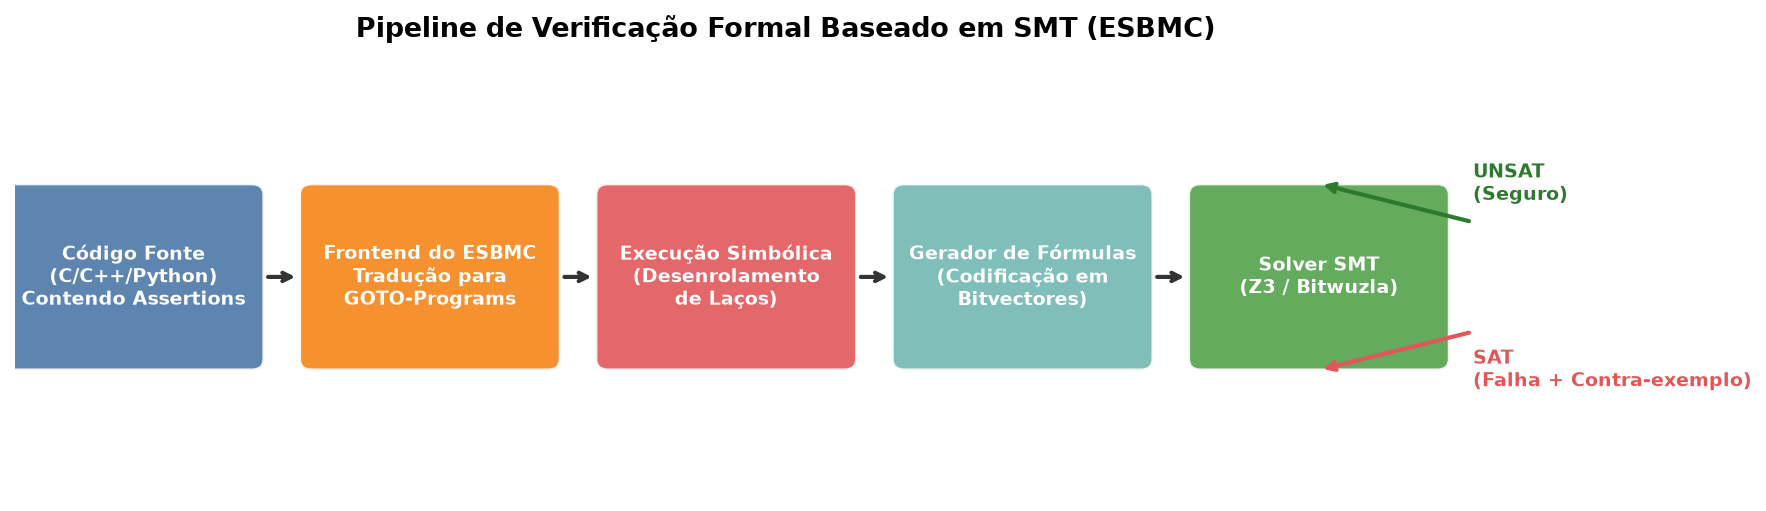
\includegraphics[width=0.92\textwidth]{fluxo-esbmc.png}
\caption{Fluxo de verificação formal com o ESBMC, do código-fonte ao veredito do
\textit{solver}.}
\label{fig:pipeline}
\legend{\small Fonte: elaborada pelo autor.}
\end{figure}

Sobre esse ciclo foram construídas três camadas metodológicas que constituem a contribuição
de infraestrutura do projeto: um invólucro programático que classifica corretamente o
resultado do verificador (Seção~\ref{sub:wrapper}), um protocolo de evidência que torna cada
número reexecutável (Seção~\ref{sub:evidencia}), e um teste de vacuidade que impede que uma
propriedade seja aceita sem que o modelo participe da prova (Seção~\ref{sub:vacuidade}).

\subsection{A camada \texttt{core\_verify} e o status tri-estado}
\label{sub:wrapper}

A automação da verificação exige interpretar a saída do ESBMC programaticamente. A primeira
implementação do projeto reduzia essa interpretação a um booleano \texttt{is\_safe}, derivado
da presença da cadeia \texttt{VERIFICATION SUCCESSFUL} na saída padrão. Essa modelagem
contém um defeito grave e silencioso: quando o verificador \emph{não executa} --- arquivo
ausente, erro de compilação, \textit{flag} inexistente, estouro de tempo ---
\texttt{is\_safe} também é falso, e o código cliente que testa \texttt{not is\_safe} conclui
``bug encontrado'' a partir de uma execução que nunca ocorreu.

O invólucro foi reescrito para derivar um status de seis valores, cruzando o código de
retorno do processo com o marcador textual da saída:

\begin{lstlisting}[language=Python,caption={Interpretação correta do resultado da verificação.},label={lst:status}]
from core_verify.esbmc_caller import run_esbmc, SAFE, UNSAFE

r = run_esbmc("harness.c", z3=True, floatbv=True, unwind=10)

r.status      # SAFE | UNSAFE | PARSE_ERROR | USAGE_ERROR | TIMEOUT | UNKNOWN
r.verificou   # True somente em SAFE ou UNSAFE

if r.status == UNSAFE:        # correto
    tratar_contraexemplo(r)
# if not r.is_safe:           # INCORRETO: verdadeiro tambem quando nada rodou
\end{lstlisting}

Quando código de retorno e marcador discordam, o status resultante é \veredito{unknown}, e
não um dos dois vereditos: a discordância indica que a execução não é confiável. Os códigos
de retorno foram medidos diretamente sobre o binário 6.8.0 utilizado (0, 1, 6 e 64). O
tratamento de \textit{timeout} encerra o grupo de processos, e não apenas o processo filho,
evitando que instâncias do \textit{solver} sobrevivam à chamada.

Duas regressões foram acrescentadas à suíte para congelar decisões que já haviam sido
tomadas erradas antes. A primeira garante que as \textit{flags} \texttt{--bounds-check} e
\texttt{--pointer-check}, que \textbf{não existem} no ESBMC --- as verificações
correspondentes são ativadas por padrão e a ferramenta expõe apenas as formas negativas ---
jamais voltem a ser emitidas; ao recebê-las, o verificador termina com código 64, que o
invólucro classifica como \veredito{usage\_error} e não como propriedade violada. A segunda
exercita os quatro modos de falha (arquivo ausente, fonte inválido, \textit{flag} inválida e
estouro de tempo) exigindo, em cada caso, que o resultado \textbf{não} seja confundido com
\veredito{unsafe}.

\subsection{Protocolo de evidência}
\label{sub:evidencia}

Todo veredito citado neste relatório é produzido por um único ponto de entrada,
\texttt{scripts/gerar\_evidencias.py}, que executa cada \textit{harness}, grava a saída
\textbf{bruta} do \textit{solver} em \texttt{results/logs/} e consolida a tabela
afirmação~$\rightarrow$~comando~$\rightarrow$~veredito~$\rightarrow$~log em
\texttt{results/EVIDENCIAS.md}. O protocolo obedece a quatro regras:

\begin{enumerate}[leftmargin=1.4cm]
  \item a saída bruta é sempre preservada, inclusive quando o veredito é negativo ou
  indeciso, e nunca filtrada por palavra-chave antes de ser gravada;
  \item \textit{timeout} é registrado como \textbf{indeciso}, em coluna distinta de
  \veredito{safe} e de \veredito{unsafe}, e nunca colapsado com nenhum dos dois;
  \item o ambiente de execução --- versão do verificador, \textit{solver}, \textit{flags}
  completas, limite de tempo, sistema operacional e número de núcleos --- acompanha cada
  medição;
  \item falha de compilação aparece como \veredito{parse\_error}, e não como ausência de
  violação.
\end{enumerate}

A Tabela~\ref{tab:ambiente} descreve o ambiente da execução consolidada reportada na
Seção~\ref{sec:resultados}.

\begin{table}[H]
\centering
\caption{Ambiente da execução consolidada de evidências.}
\label{tab:ambiente}
\small
\begin{tabular}{@{}ll@{}}
\toprule
\textbf{Item} & \textbf{Valor} \\
\midrule
Verificador            & ESBMC 6.8.0, 64 bits, \texttt{x86\_64-linux} \\
\textit{Solvers}       & Boolector (padrão) e Z3 (\textit{harnesses} com \texttt{--floatbv}) \\
Sistema operacional    & Linux 6.18.5, \texttt{x86\_64}, glibc 2.39 \\
Processador            & 4 núcleos \\
\textit{Harnesses}     & 12, todos reexecutáveis por \texttt{scripts/gerar\_evidencias.py} \\
Duração total          & 463\,s \\
\bottomrule
\end{tabular}
\legend{\small Fonte: \texttt{results/EVIDENCIAS.md}, gerado por execução.}
\end{table}

Registre-se que o binário versionado no repositório é a versão 6.8.0, enquanto a árvore de
código do ESBMC presente no mesmo repositório é a 8.0.0, não compilada. Algumas
\textit{flags} existem apenas nesta última --- entre elas \texttt{--std}, necessária para
C++11, \texttt{--multi-property} e \texttt{--cvc4}. Essa diferença é a causa direta de dois
bloqueios reportados na Seção~\ref{sec:resultados}.

\subsection{Teste de vacuidade}
\label{sub:vacuidade}

Uma propriedade é \textbf{vácua} quando seu veredito não depende do artefato que se pretende
verificar. O teste adotado é direto e barato: substitui-se o modelo por uma entrada livre e
reexecuta-se a mesma asserção. Se o veredito e o contraexemplo se reproduzem inalterados, o
modelo era código morto para aquela propriedade.

O procedimento é aplicado em duas direções complementares:

\begin{itemize}[leftmargin=1.4cm]
  \item \textbf{vacuidade do modelo}: a rede é removida e a propriedade reexecutada. Se ainda
  decide, ela não fala sobre a rede;
  \item \textbf{vacuidade das hipóteses}: insere-se \texttt{assert(0)} imediatamente após os
  \texttt{assume} do \textit{harness}. Se essa asserção for \emph{provada}, os \texttt{assume}
  são insatisfazíveis e todo veredito daquele \textit{harness} é vazio.
\end{itemize}

Aplicado às propriedades da malha fechada, o teste revelou duas vacuidades, cuja correção é
relatada na Seção~\ref{sub:cartpole}. Aplicado às 24 hipóteses da segunda camada da rede de
neurônios mortos, mostrou que nenhum \texttt{assume} é insatisfazível --- o risco existia,
mas não se materializou naquele conjunto.

\subsection{Formulação dos estudos de caso}

\subsubsection{Caso 1 --- rede neural quantizada e \textit{stubs} de inferência}

Uma perceptron multicamadas com ativação ReLU foi implementada em ponto fixo Q8.8, com as
operações \texttt{fxp\_add} e \texttt{fxp\_mult} reproduzindo o truncamento do dispositivo
alvo, e verificada sobre as quatro entradas discretas do problema XOR. Ao lado dela, foram
verificados um \textit{stub} da mesma rede em ponto flutuante, um \textit{harness} de
propriedade sobre a rede completa e um \textit{stub} de bloco MLP \textit{gated} no estilo
DeepSeek. A pré-condição de entrada é $x_1, x_2 \in [0,1]$ e a propriedade de saída é um
limite superior explícito sobre a predição desquantizada.

Neste caso foi reproduzida, em código, a estratégia de poda por intervalos do QNNVerifier:
limites por neurônio são injetados como hipóteses, colapsando ramos que a propagação de
valores mostra inalcançáveis. A operação é uma \emph{sobreaproximação} e está declarada como
tal --- o veredito vale para a relaxação definida pelos intervalos.

\subsubsection{Caso 2 --- \textit{kernels} de inferência em C/C++}

Dois \textit{kernels} análogos aos de motores de inferência foram verificados quanto a
segurança de memória: um \textit{kernel} de atenção por produto escalar com alocação dinâmica
e comprimento de sequência simbólico $\texttt{seq\_len} \in [1,10]$, e um \textit{kernel} de
multiplicação de matrizes com \textit{tiling}, parametrizado pela dimensão $N$ para o estudo
de escalabilidade. As verificações empregam \texttt{--memory-leak-check} e
\texttt{--overflow-check}, com limite de tempo de 300\,s.

\subsubsection{Caso 3 --- ciclo neuro-simbólico de geração e correção}

O terceiro caso modela o protocolo em que um gerador produz código C, o ESBMC o verifica e,
havendo contraexemplo, o diagnóstico volta ao gerador como entrada para correção. A
iteração~0 introduz deliberadamente um \textit{buffer overflow} por \texttt{strcpy} de 20
bytes em um destino de 10; a iteração~1 aplica a correção com \texttt{strncpy}.

O gerador é um \textbf{\textit{mock} determinístico}, e não um modelo de linguagem. Essa
escolha é uma limitação assumida do experimento e está registrada como tal: o que se
demonstra é o protocolo e o custo do verificador dentro do ciclo, não a competência de um
agente autônomo.

\subsubsection{Caso 4 --- controlador PID sob ruído não determinístico}

Uma planta térmica de primeira ordem, com aquecimento proporcional à ação de controle e perda
constante, é regulada por um PID digital com $K_p = 1{,}0$, $K_i = 0{,}1$, $K_d = 0{,}5$ e
saturação em $[0, 100]$:

\begin{equation}
T_{k+1} = \max\!\left(20,\; T_k + (u_k r_h - r_c)\,\Delta t\right), \qquad
u_k = K_p e_k + K_i \sum_{j \le k} e_j \Delta t + K_d \frac{e_k - e_{k-1}}{\Delta t}.
\end{equation}

O ruído de sensor é escolhido pelo próprio \textit{solver} a cada passo, restrito a
$[-5,+5]\,^\circ$C, e a propriedade de segurança é a invariante $T_k < 150\,^\circ$C para
todos os dez passos. A verificação usa \texttt{--floatbv} e \texttt{--unwind 11}.

Complementarmente, avaliou-se a aplicabilidade da abordagem a uma biblioteca de controle real
de terceiros: a \textit{Arduino-PID-Library}, incorporada como submódulo Git fixado em
\textit{commit} determinado, com \textit{harness} que instancia a classe \texttt{PID} sob a
mesma planta e o mesmo modelo de ruído.

\subsubsection{Caso 5 --- blocos \textit{feed-forward} de modelos de linguagem}

Blocos FFN foram extraídos de modelos ONNX do GPT-2 e do LLaMA-7B e quantizados em Q8.8. Duas
codificações foram comparadas:

\begin{itemize}[leftmargin=1.4cm]
  \item \textbf{Método 1 --- \textit{proxy} ReLU}: substitui GeLU/SiLU por ReLU. É mais
  rápido, mas verifica um modelo que não é o modelo implantado;
  \item \textbf{Método 2 --- ativação abstrata}: substitui a ativação por hipóteses de
  intervalo por neurônio, no estilo do QNNVerifier. Produz uma sobreaproximação intervalar,
  conservadora \emph{somente se} os limites cobrirem todas as saídas alcançáveis; a relação
  funcional exata não é codificada.
\end{itemize}

Os resultados reportados adiante correspondem ao Método 2. Os geradores de
\textit{harnesses} e as tabelas de consulta de GeLU e SiLU são reexecutáveis e produzem
arquivos byte a byte idênticos aos versionados.

A dificuldade de fundo é que $\sigma(z) = 1/(1+e^{-z})$ é transcendental e não possui
axiomatização SMT, levando a \veredito{unknown}. Onde foi necessário manter a forma
funcional, empregou-se a aproximação linear conservadora
$\sigma_{\text{aprox}}(z) = \operatorname{clip}(0{,}25z + 0{,}5,\,0,\,1)$, tangente de
$\sigma$ em $z = 0$ com saturação, ilustrada na Figura~\ref{fig:silu}.

\begin{figure}[H]
\centering
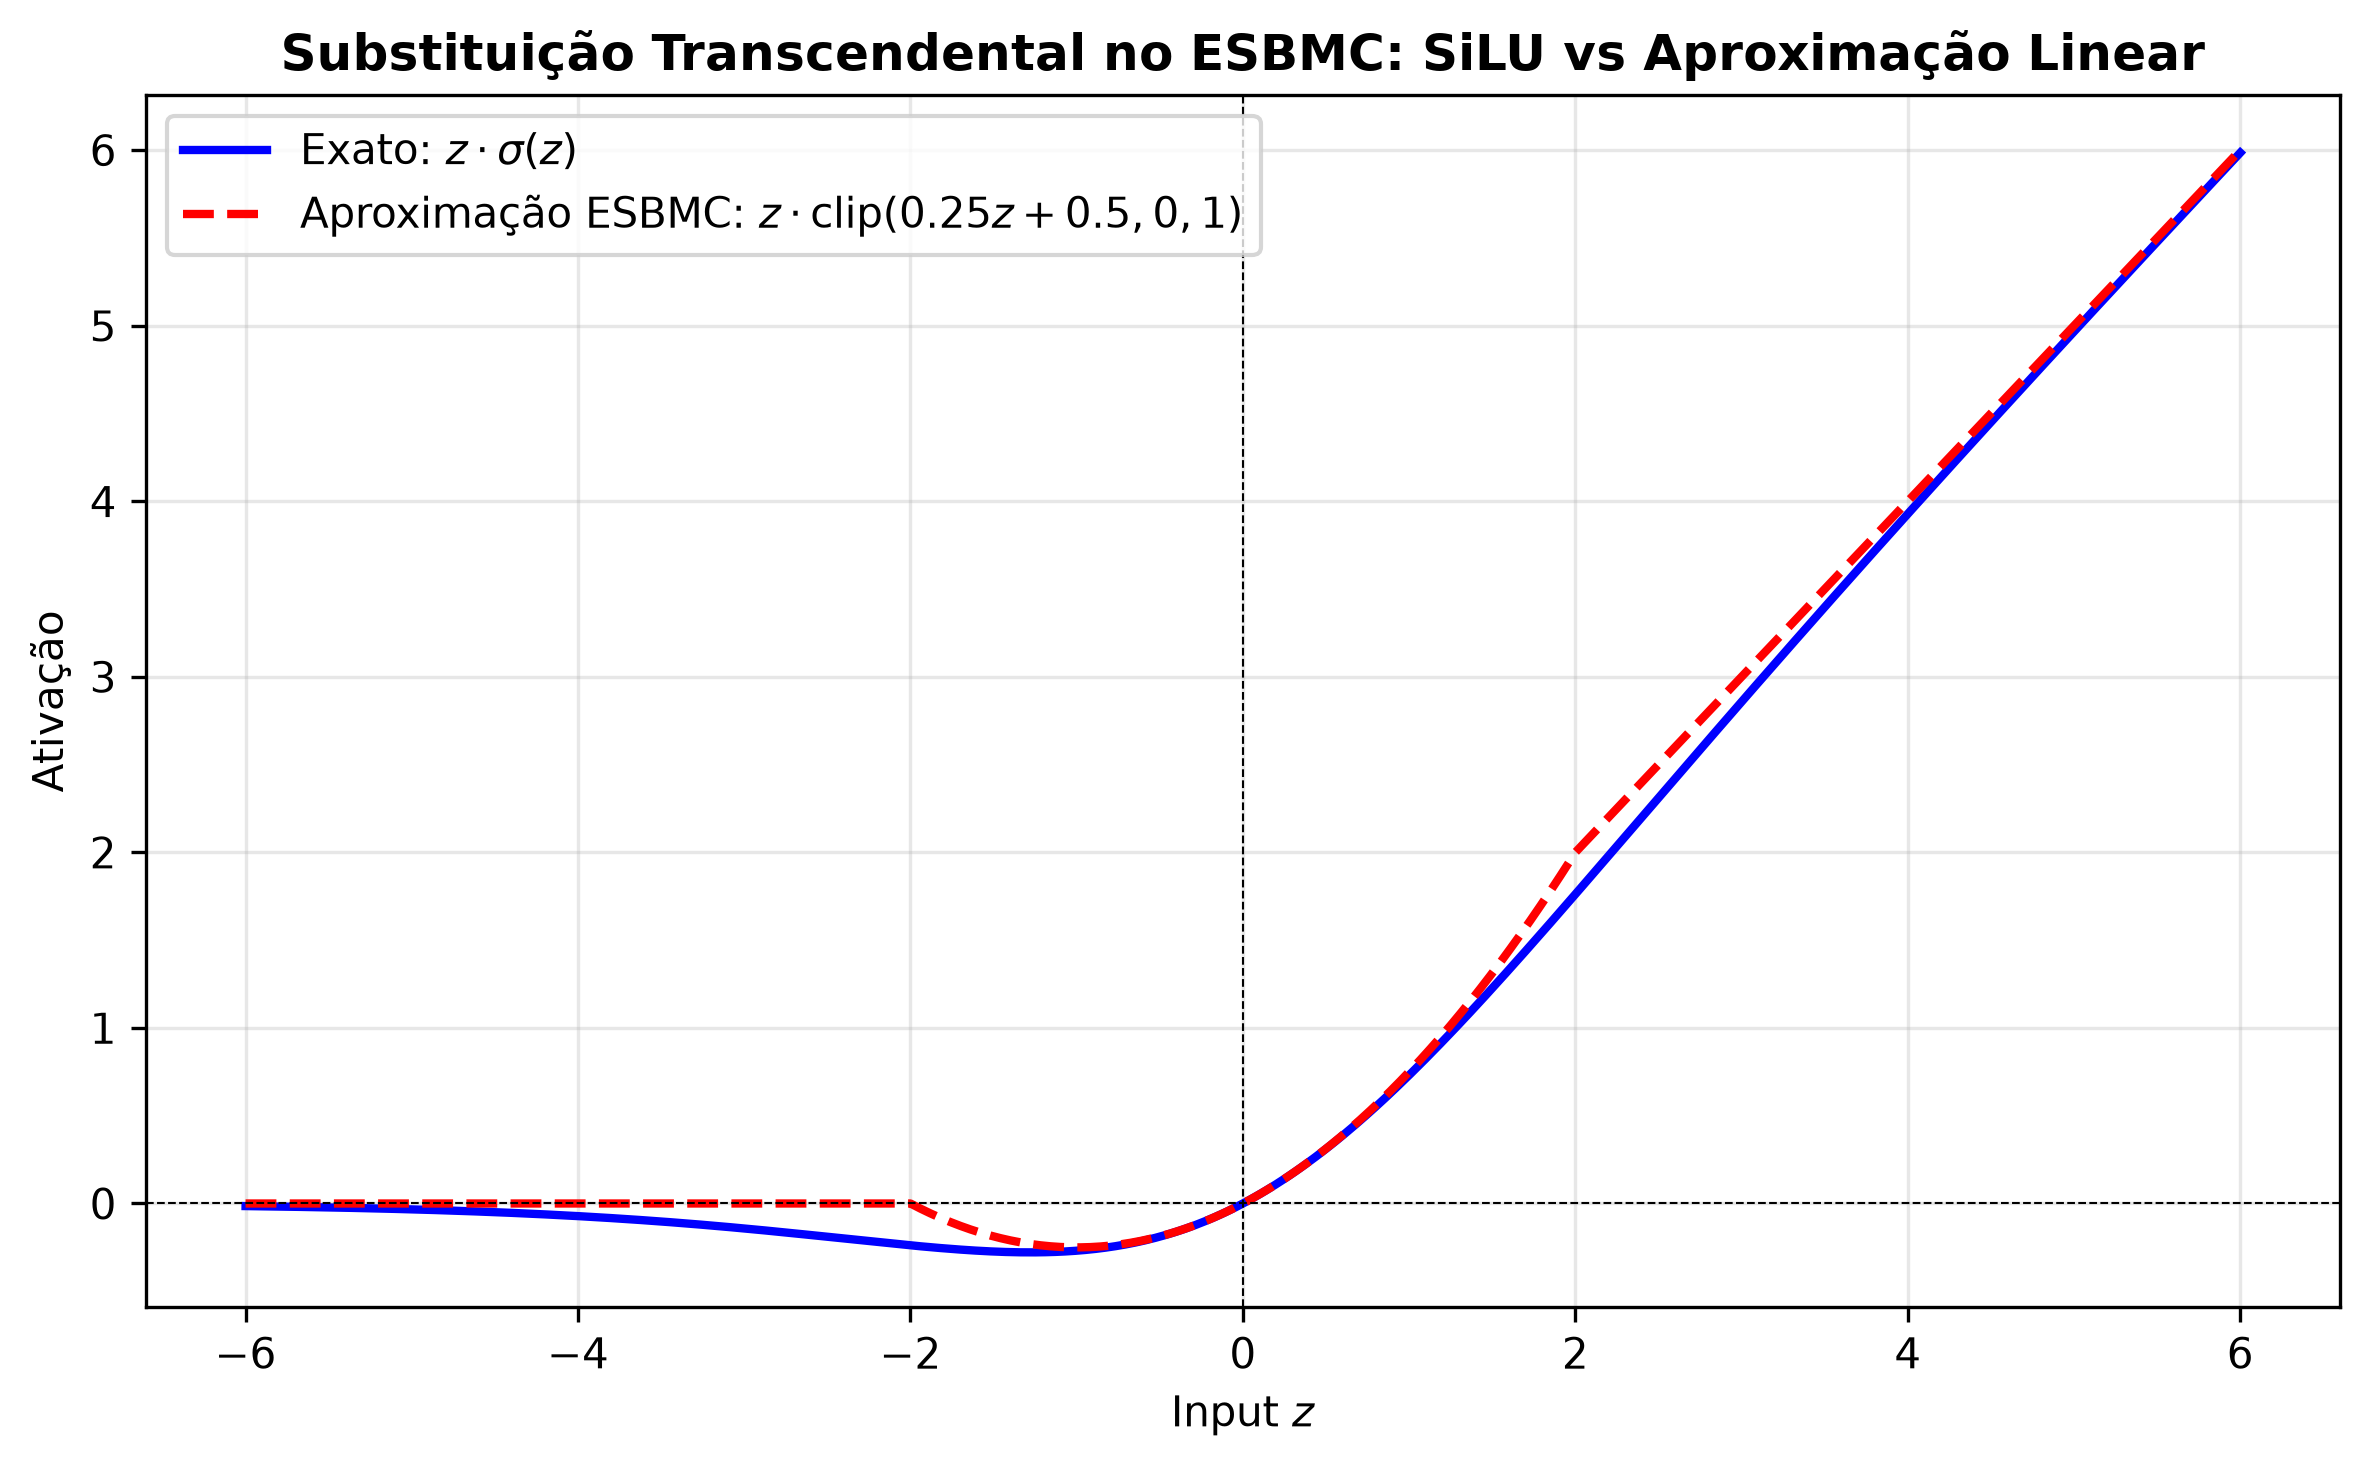
\includegraphics[width=0.86\textwidth]{plot_silu_approx.png}
\caption{Substituição da ativação transcendental: SiLU exata contra a aproximação linear
tratável pelo \textit{solver}. O veredito obtido vale para a aproximação, não para a função
original.}
\label{fig:silu}
\legend{\small Fonte: elaborada pelo autor.}
\end{figure}

\subsubsection{Caso 6 --- política de aprendizado por reforço}

Uma política de RL do tipo ator-crítico, com ação contínua em $[-1,1]$, foi transcrita para C
e submetida à busca não determinística sob \texttt{--floatbv}, com o objetivo de decidir se
existe estado, dentro da caixa admitida, para o qual a ação viola o limite do atuador.

\subsubsection{Caso 7 --- malha fechada \textit{cart-pole} com controlador DDPG}
\label{sub:metodologia_cartpole}

Este é o único caso em que planta e controlador são verificados \textbf{acoplados}. O ator
DDPG \cite{lillicrap2016ddpg}, de arquitetura $4 \rightarrow 24 \rightarrow 24 \rightarrow 1$
e 745 parâmetros, foi quantizado em Q8.8 e integrado ao modelo do \textit{cart-pole}
\cite{barto1983cartpole}. A aritmética de inferência está implementada três vezes --- em
Python para o treinamento, em TypeScript para a demonstração em navegador e em C para o
\textit{harness} --- e as três coincidem bit a bit: mesma ordem de operações, mesmo
truncamento em direção a zero e mesma aproximação de $\tanh$ em cinco ramos.

Para superar o horizonte do BMC, o sistema acoplado foi também exportado como sistema de
transição: \texttt{gen\_transition\_system.py} lê os pesos reais e emite Verilog com largura
configurável, o Yosys \cite{wolf2016yosys} sintetiza o circuito e o ABC
\cite{brayton2010abc} executa \texttt{pdr} e \texttt{bmc3}. Antes de qualquer medição,
\texttt{validate\_forward.py} realiza um teste diferencial entre o Verilog gerado e a
referência Q8.8 em doze estados amostrados; a coincidência detecta regressão de tradução, mas
\textbf{não} constitui prova de equivalência universal entre as implementações.

\subsection{Integração contínua}

A suíte de verificação é executada a cada submissão por um fluxo de integração contínua. Duas
decisões de projeto merecem registro por decorrerem de defeitos observados na primeira versão
do fluxo. O binário do verificador é \textbf{versionado junto ao repositório} em vez de
baixado a cada execução, o que elimina a divergência de versão entre ambiente local e remoto
--- fonte de resultados não reproduzíveis. E o caminho do binário é propagado por
\texttt{\$GITHUB\_ENV}, e não por \texttt{export PATH}: variáveis exportadas em um passo não
persistem para o seguinte, defeito que mantinha a etapa de verificação inoperante \emph{sem
emitir erro}.

Por decisão de escopo do ciclo, os resultados de execução remota em múltiplas plataformas
não são apresentados como evidência neste relatório. A aceitação dos resultados apoia-se
exclusivamente nas execuções locais documentadas na Seção~\ref{sec:resultados}; a
estabilização em Windows, macOS e ARM permanece como trabalho separado.

% =====================================================================
\section{Resultados e discussão}
\label{sec:resultados}

\subsection{Consolidado das evidências}

A Tabela~\ref{tab:evidencias} apresenta o resultado da execução consolidada dos doze
\textit{harnesses} citados neste relatório. Cada linha corresponde a um arquivo de log bruto
versionado, indexado no Apêndice~B. O ambiente é o da
Tabela~\ref{tab:ambiente}.

\begin{table}[H]
\centering
\caption{Vereditos medidos dos doze \textit{harnesses} reexecutáveis.}
\label{tab:evidencias}
\footnotesize
\begin{tabular}{@{}llcr@{}}
\toprule
\textbf{Caso} & \textbf{\textit{Harness}} & \textbf{Veredito} & \textbf{Tempo} \\
\midrule
Caso 1 & MLP quantizada (XOR), Q8.8             & \SAFE   & 0,08\,s \\
Caso 1 & \textit{Stub} da MLP em ponto flutuante & \SAFE   & 3,09\,s \\
Caso 1 & Rede completa + propriedade de saída    & \UNSAFE & 197,82\,s \\
Caso 1 & \textit{Stub} de bloco MLP \textit{gated} & \SAFE & 0,08\,s \\
Caso 2 & \textit{Kernels} de inferência          & \UNSAFE & 0,43\,s \\
Caso 2 & GEMM com \textit{tiling}, $N=3$         & \SAFE   & 17,51\,s \\
Caso 4 & PID, ruído $[-5,+5]$, 10 passos         & \SAFE   & 213,47\,s \\
Caso 6 & Política de RL, limite do atuador       & \UNSAFE & 2,58\,s \\
Caso 5 & FFN GPT-2 $2{\times}4$, intervalo GeLU  & \SAFE   & 0,24\,s \\
Caso 5 & FFN LLaMA-7B $4{\times}8$, intervalo SiLU & \SAFE & 3,46\,s \\
Caso 5 & FFN GPT-2 $4{\times}8$, intervalo GeLU  & \SAFE   & 4,24\,s \\
Caso 5 & FFN GPT-2 $4{\times}16$, intervalo GeLU & \SAFE   & 20,10\,s \\
\midrule
\multicolumn{4}{@{}l@{}}{\textbf{9 provados $\cdot$ 3 com contraexemplo $\cdot$ 0 indecisos}} \\
\bottomrule
\end{tabular}
\legend{\small Fonte: \texttt{results/EVIDENCIAS.md}; logs brutos em \texttt{results/logs/}.}
\end{table}

Três leituras equivocadas dessa tabela precisam ser bloqueadas de antemão. Um veredito
\SAFE{} vale para o \textit{harness}, para as hipóteses declaradas e para o horizonte de
desenrolamento indicado, e não para o sistema implantado. Um veredito \UNSAFE{} é um
resultado positivo do ponto de vista da verificação --- o \textit{solver} exibiu um traço
concreto ---, e não uma falha do experimento. E a ausência de linhas indecisas nesta execução
específica não significa que a técnica sempre decida: várias configurações estudadas neste
projeto \textbf{não} decidem, e estão reportadas nas subseções seguintes.

\subsection{Caso 1 --- redes quantizadas e \textit{stubs} de inferência}

O \textit{harness} C quantizado que implementa XOR sobre as quatro entradas discretas foi
provado em 0,08\,s, e o \textit{stub} em ponto flutuante da mesma topologia em 3,09\,s. O
\textit{stub} de bloco MLP \textit{gated}, no estilo DeepSeek, gera 28 condições de
verificação --- quatro remanescentes após simplificação --- e é provado em 0,08\,s.

Já o \textit{harness} que impõe a propriedade de saída sobre a rede completa em ponto
flutuante retorna \UNSAFE{} em 197,82\,s: existe entrada admissível para a qual a predição
desquantizada excede o limite declarado. Esse resultado é informativo justamente por
contrariar a expectativa induzida pela amostragem. A Figura~\ref{fig:case1} mostra a
superfície de saída obtida por amostragem densa de $10^4$ pontos, em que nenhuma violação
aparece --- um lembrete direto de que $10^4$ amostras não cobrem um domínio contínuo, e de
que a diferença entre ``não encontrei'' e ``não existe'' é exatamente o que a verificação
formal entrega.

\begin{figure}[H]
\centering
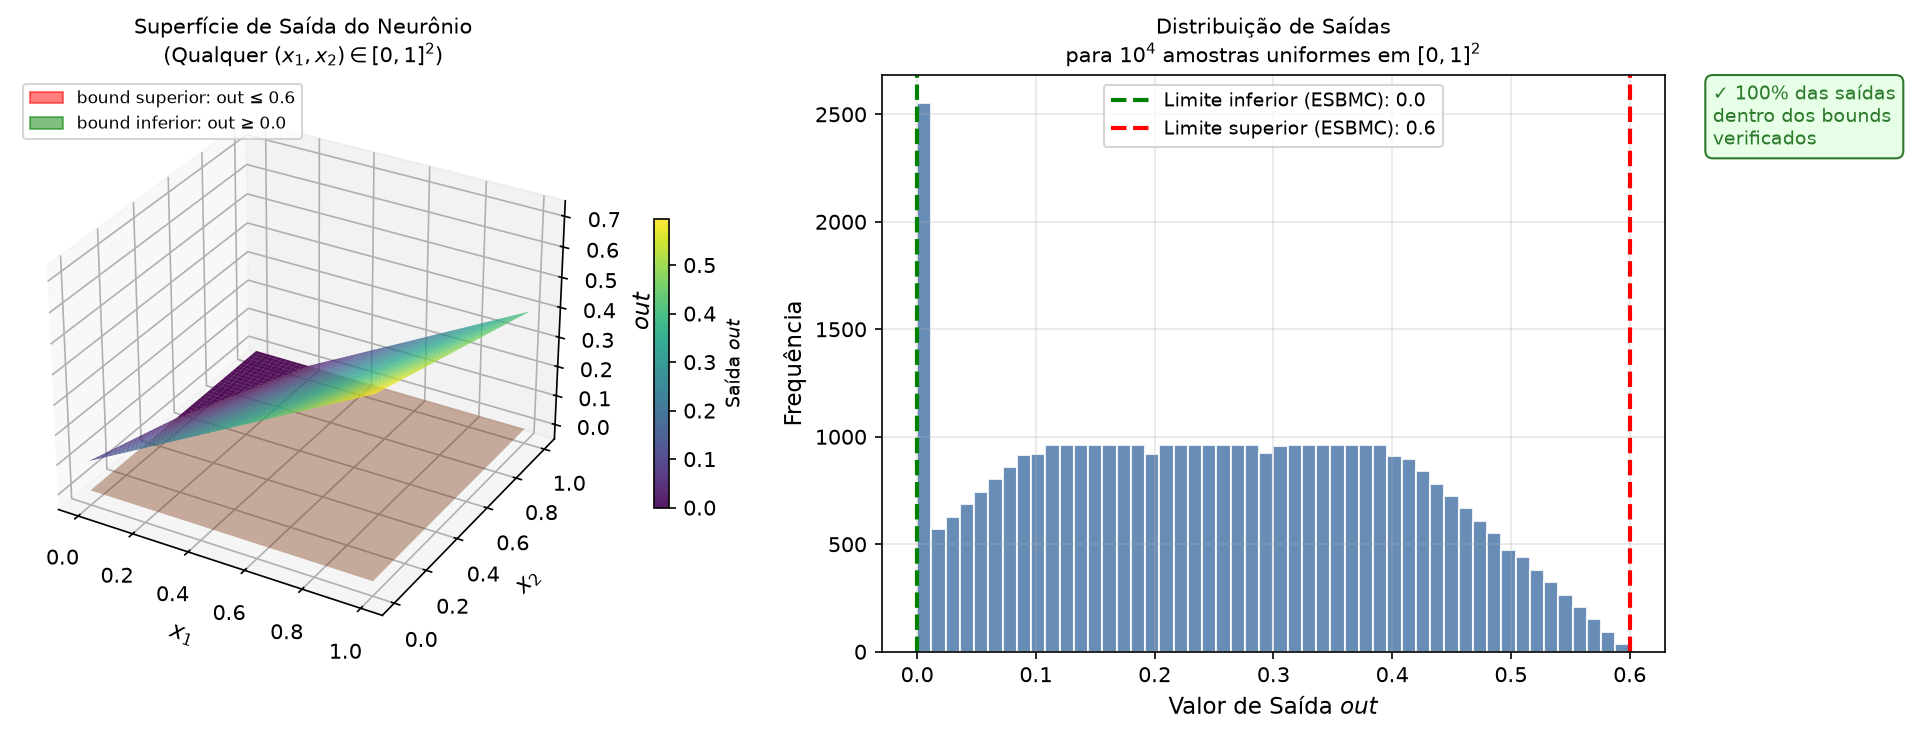
\includegraphics[width=0.90\textwidth]{case1_plot.png}
\caption{Superfície de saída do neurônio e distribuição amostral. A figura descreve a
amostra e \textbf{não} constitui prova sobre o domínio contínuo.}
\label{fig:case1}
\legend{\small Fonte: elaborada pelo autor.}
\end{figure}

Registre-se um limite de escopo desta frente. O plano previa executar a verificação
diretamente sobre o modelo em Python, via \texttt{esbmc modelo.py --floatbv --k-induction}. O
binário 6.8.0 versionado no repositório não possui o \textit{frontend} Python compilado e
rejeita arquivos \texttt{.py} com \texttt{failed to figure out type of file}; instalar as
dependências de transpilação não contorna o problema, pois a limitação está no binário.
Concluir esse experimento exige compilar a versão 8.0.0 com
\texttt{-DENABLE\_PYTHON\_FRONTEND=ON}. Nenhum veredito é atribuído aqui ao modelo em Python.

\subsection{Caso 2 --- \textit{kernels} de inferência e a barreira de escalabilidade}

A verificação dos \textit{kernels} de inferência produziu contraexemplo em 0,43\,s,
localizando violação de segurança de memória sob comprimento de sequência simbólico. Para o
\textit{kernel} GEMM com \textit{tiling}, a Tabela~\ref{tab:gemm} apresenta o estudo de
escalabilidade.

\begin{table}[H]
\centering
\caption{Escalabilidade da verificação do \textit{kernel} GEMM em função da dimensão $N$.}
\label{tab:gemm}
\small
\begin{tabular}{@{}crl@{}}
\toprule
\textbf{Dimensão $N$} & \textbf{Tempo} & \textbf{Veredito} \\
\midrule
2 & 1,97\,s   & \SAFE \\
3 & 16,83\,s  & \SAFE \\
4 & 300,05\,s & \INDECISO{} (indeciso) \\
\bottomrule
\end{tabular}
\legend{\small Fonte: \texttt{results/case2\_ambiente.md}; Boolector, limite de 300\,s,
\texttt{-DDIM\_LIMIT=N}.}
\end{table}

De $N{=}2$ para $N{=}3$ o tempo cresce cerca de 8,5 vezes; em $N{=}4$ o \textit{solver} não
decide dentro do limite. A barreira observada, neste \textit{harness} e nesta máquina, está
em $N{=}4$. Três pontos --- um deles indeciso --- não sustentam extrapolação para dimensões
de produção nem a proposição de uma lei de crescimento, e a conclusão permanece restrita ao
experimento medido. A abordagem continua útil para verificar a corretude lógica do algoritmo
de \textit{tiling} em instâncias reduzidas, o que é coerente com a hipótese de escopo pequeno
usualmente invocada nesse contexto.

Cabe registrar como esse resultado foi obtido, porque o percurso é instrutivo. A versão
anterior do experimento reportava uma curva de seis pontos, com tempos entre $<1$\,s e
$\approx 15$\,s. O \textit{script} de execução passava a dimensão por
\texttt{-DDIM\_LIMIT=<n>}, mas o \textit{kernel} \textbf{nunca usava esse macro}: as
dimensões estavam fixas em $M = N = K = 2$, e todos os ``tamanhos'' mediam o mesmo problema.
Além disso, a \textit{flag} \texttt{--smtlib} fazia o verificador \emph{emitir} a fórmula em
vez de resolvê-la. Corrigidos o macro, a extensão do arquivo e as \textit{flags}, a curva
suave desapareceu e a barreira em $N{=}4$ tornou-se visível.

\subsection{Caso 3 --- ciclo neuro-simbólico de geração e correção}

O ciclo completou-se em \textbf{duas} iterações. Na iteração~0, o ESBMC detectou o
\textit{buffer overflow} do \texttt{strcpy} em 0,13\,s de tempo de verificador, devolvendo o
deslocamento exato da violação; na iteração~1, o código corrigido com \texttt{strncpy}
recebeu \veredito{verification successful} em 0,11\,s, encerrando o ciclo. As
Figuras~\ref{fig:case3} e~\ref{fig:statemachine} apresentam a decomposição de tempo por
iteração e a máquina de estados do protocolo.

\begin{figure}[H]
\centering
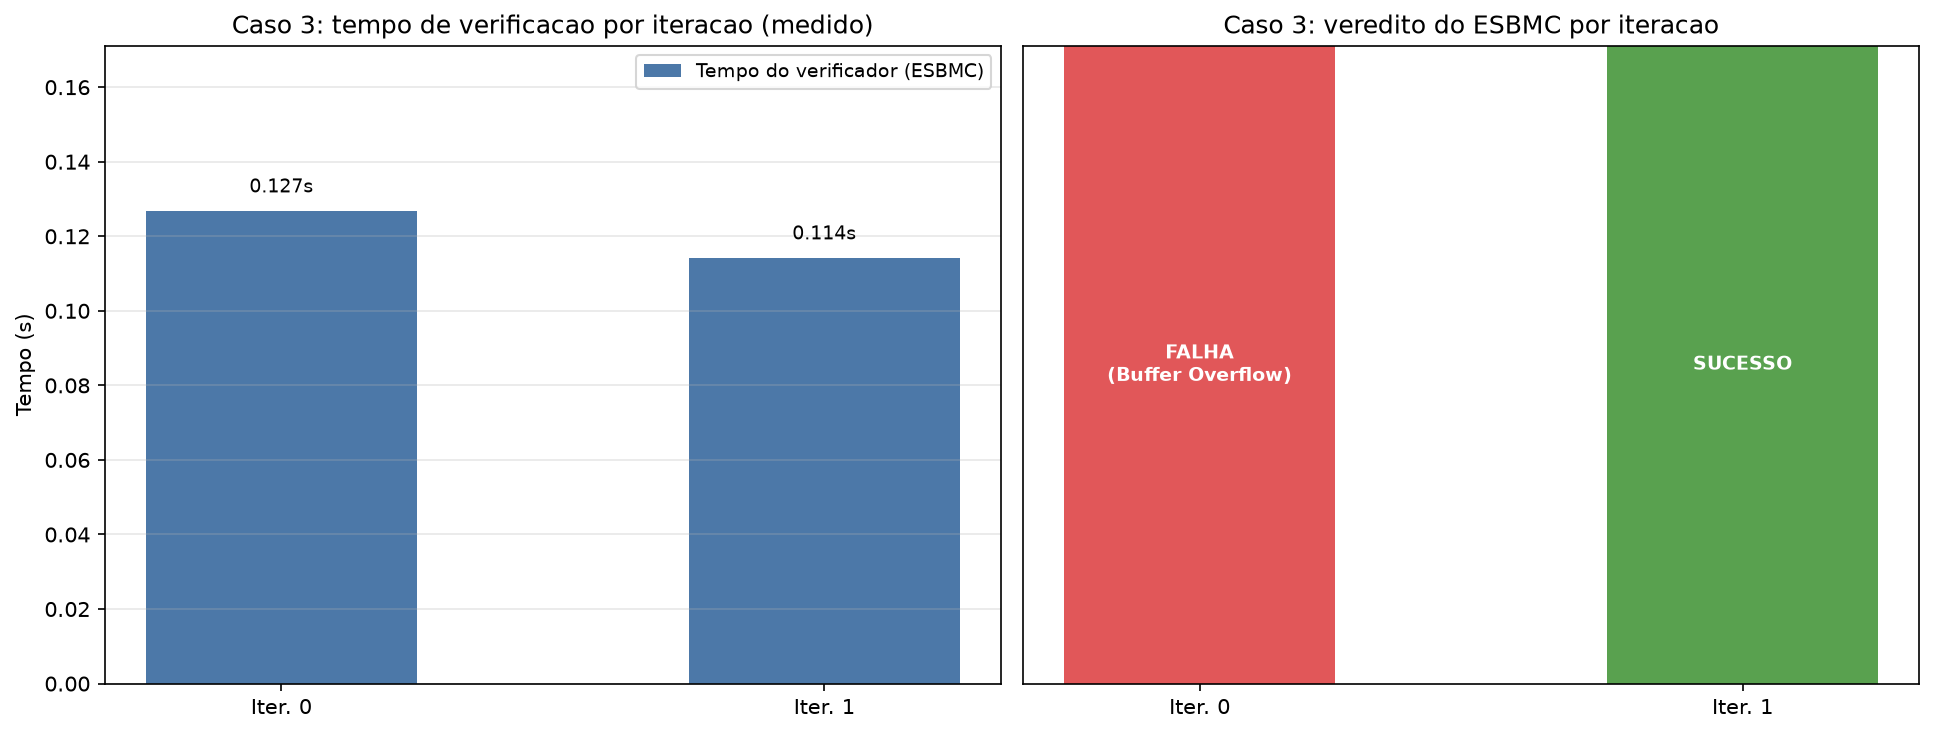
\includegraphics[width=0.95\textwidth]{case3_plot.png}
\caption{Tempo por iteração do ciclo gerar--verificar--corrigir, com decomposição entre
atraso do gerador e tempo de verificação.}
\label{fig:case3}
\legend{\small Fonte: elaborada pelo autor a partir de
\texttt{results/case3\_agent\_stats.csv}.}
\end{figure}

\begin{figure}[H]
\centering
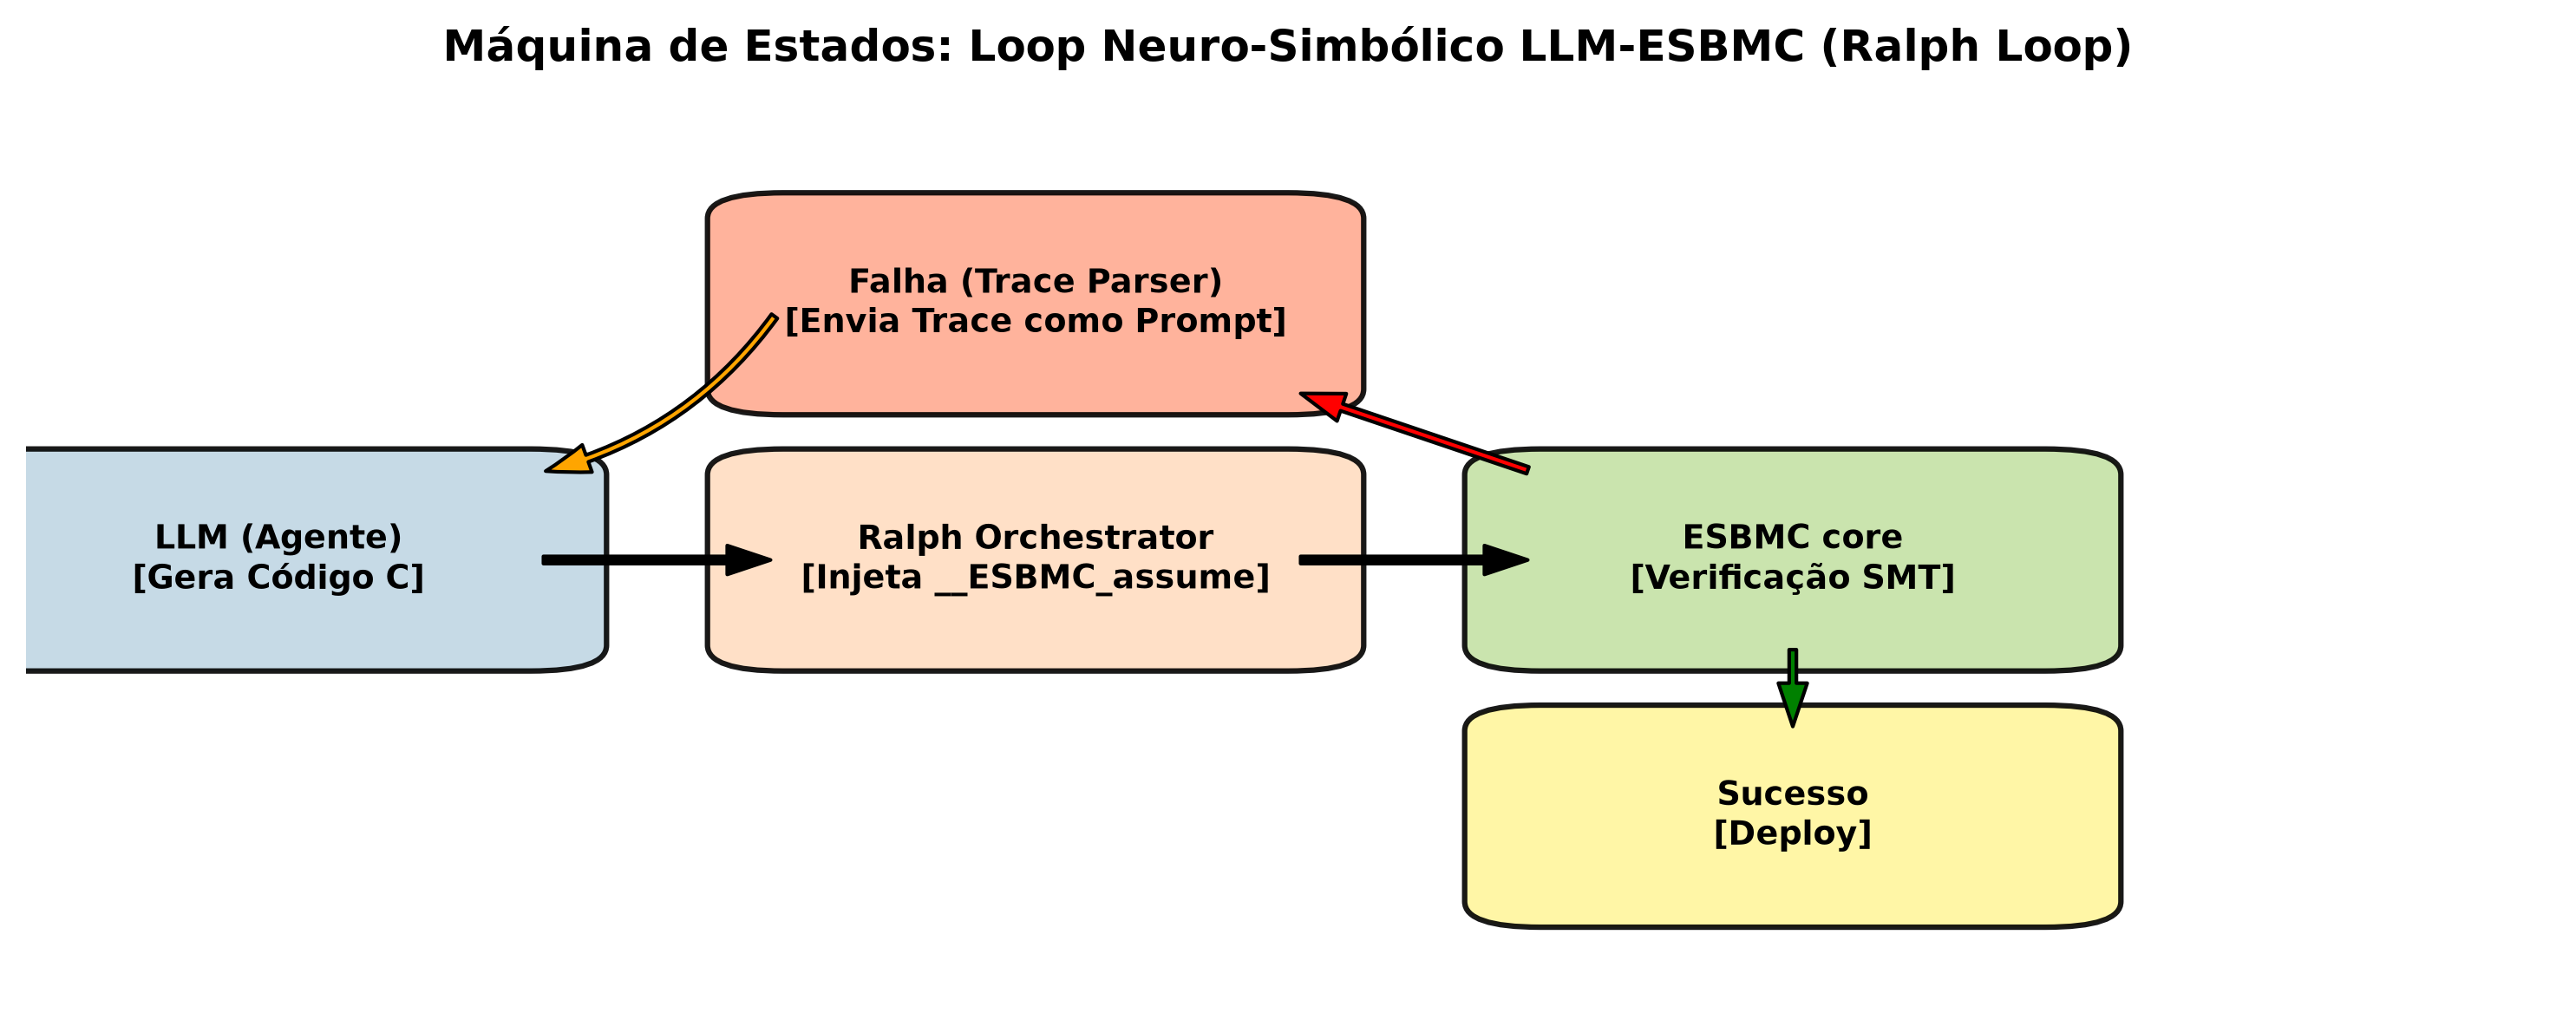
\includegraphics[width=0.88\textwidth]{plot_agent_statemachine.png}
\caption{Máquina de estados do protocolo neuro-simbólico de geração e reparo.}
\label{fig:statemachine}
\legend{\small Fonte: elaborada pelo autor.}
\end{figure}

O custo do verificador ficou abaixo de 0,15\,s nas duas iterações, mas esse número só foi
obtido após limitar o desenrolamento com \texttt{--unwind 32}: sem esse limite, o modelo de
\texttt{strncpy} não termina; com \texttt{--no-unwinding-assertions}, o caso pode tornar-se
vácuo. É um exemplo concreto de como um parâmetro aparentemente operacional altera o
significado do veredito.

Duas correções foram necessárias para que este caso medisse alguma coisa. A versão anterior
afirmava cinco iterações --- inalcançáveis, já que o ciclo encerra na primeira prova
bem-sucedida --- e usava \texttt{--smtlib}, o que fazia com que o campo de sucesso fosse
permanentemente falso e o arquivo de estatísticas ficasse com zero byte. O experimento
reportado aqui usa o invólucro \texttt{core\_verify} e produz o CSV de onde a
Figura~\ref{fig:case3} é gerada.

Reafirme-se a limitação de escopo: o gerador é um \textit{mock} determinístico. O experimento
demonstra o protocolo e mede o custo do verificador dentro dele; conclusões sobre autonomia,
qualidade de \textit{prompts} ou desempenho de agentes reais exigem outro experimento.

\subsection{Caso 4 --- PID sob ruído não determinístico}

O verificador provou, em \textbf{213,47\,s}, que o controlador mantém $T < 150\,^\circ$C ao
longo dos dez passos e para \emph{qualquer} ruído de sensor em $[-5,+5]$. A
Figura~\ref{fig:case4} apresenta a dinâmica simulada sob cinco perfis distintos de ruído e a
Figura~\ref{fig:fase} o retrato de fase correspondente.

\begin{figure}[H]
\centering
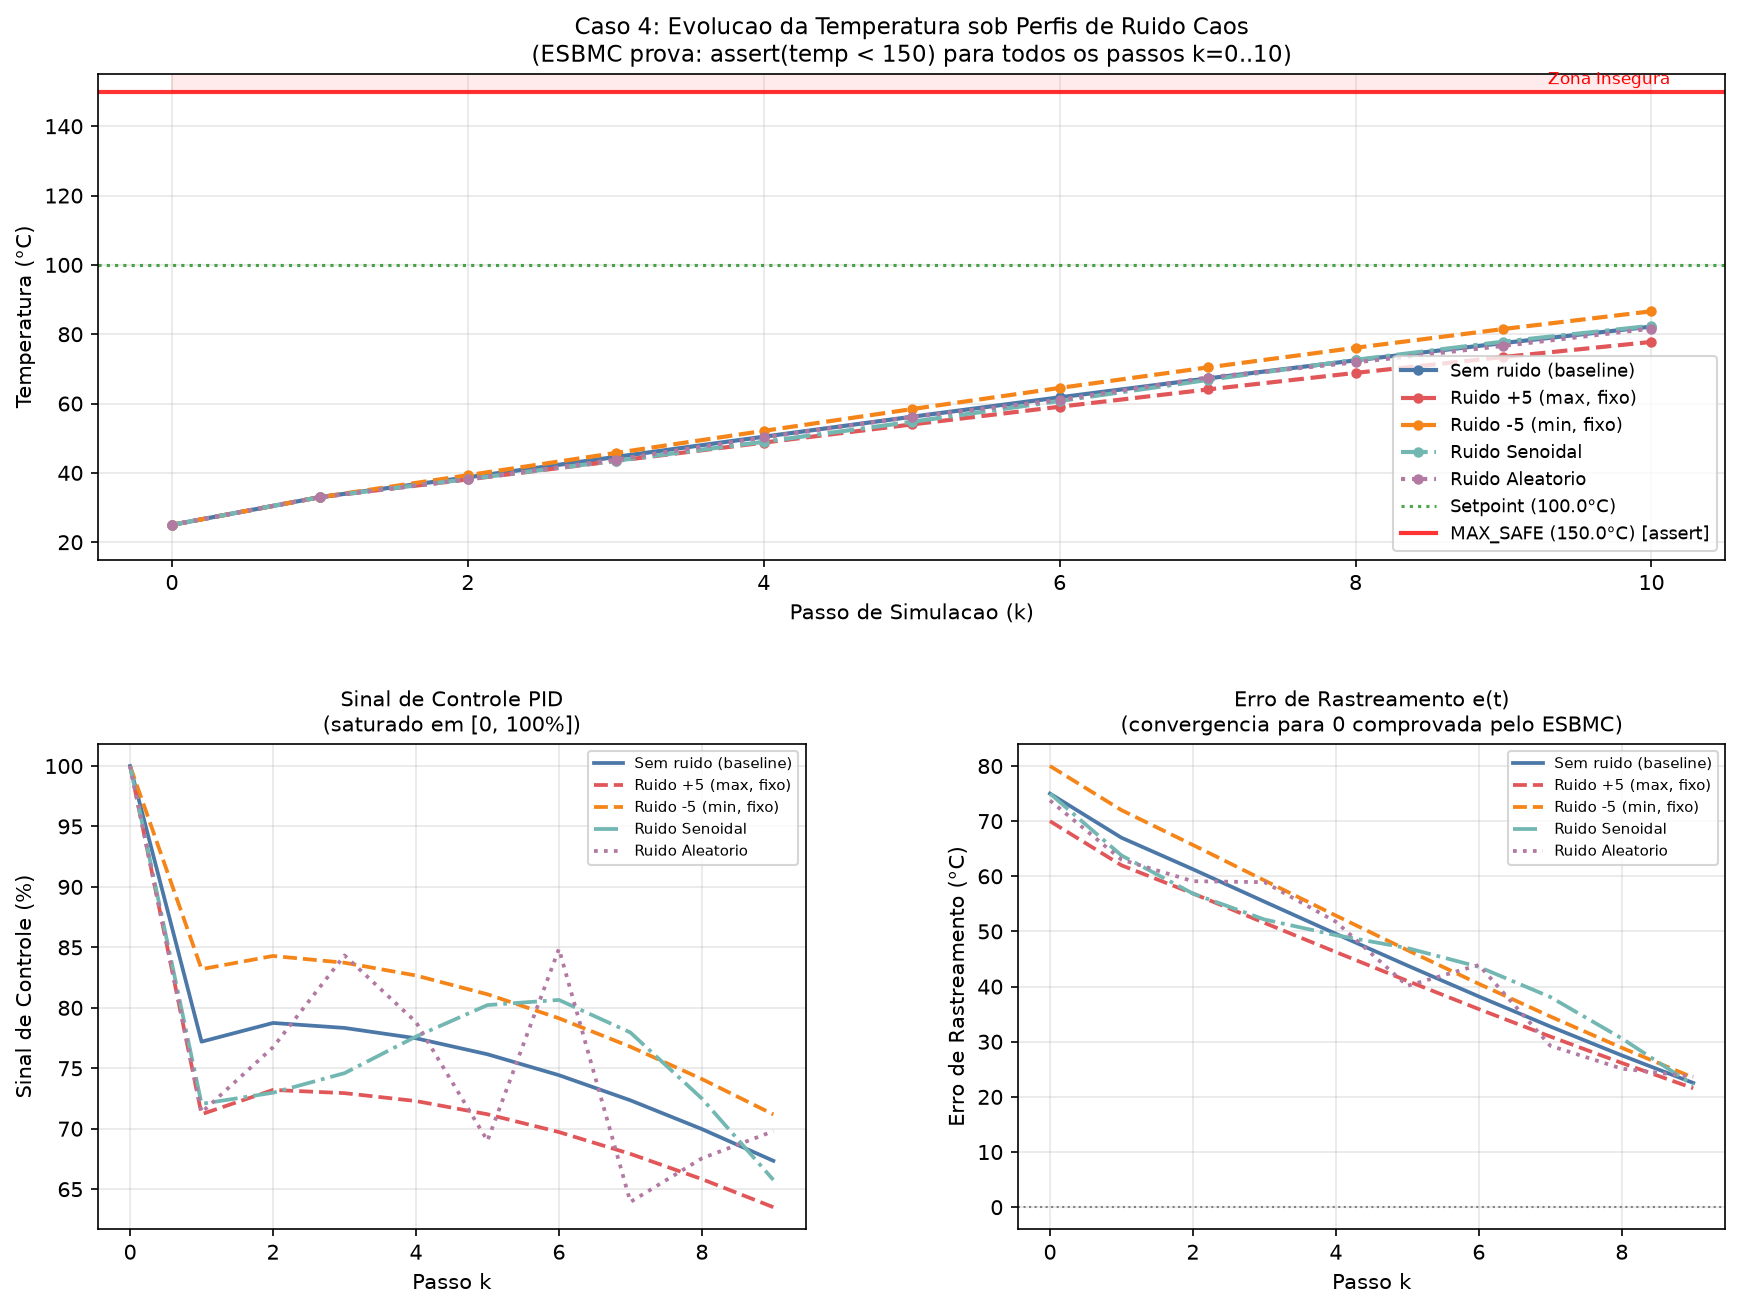
\includegraphics[width=0.95\textwidth]{case4_plot.png}
\caption{Evolução da temperatura, do sinal de controle e do erro de rastreamento sob cinco
perfis simulados de ruído de sensor.}
\label{fig:case4}
\legend{\small Fonte: elaborada pelo autor.}
\end{figure}

\begin{figure}[H]
\centering
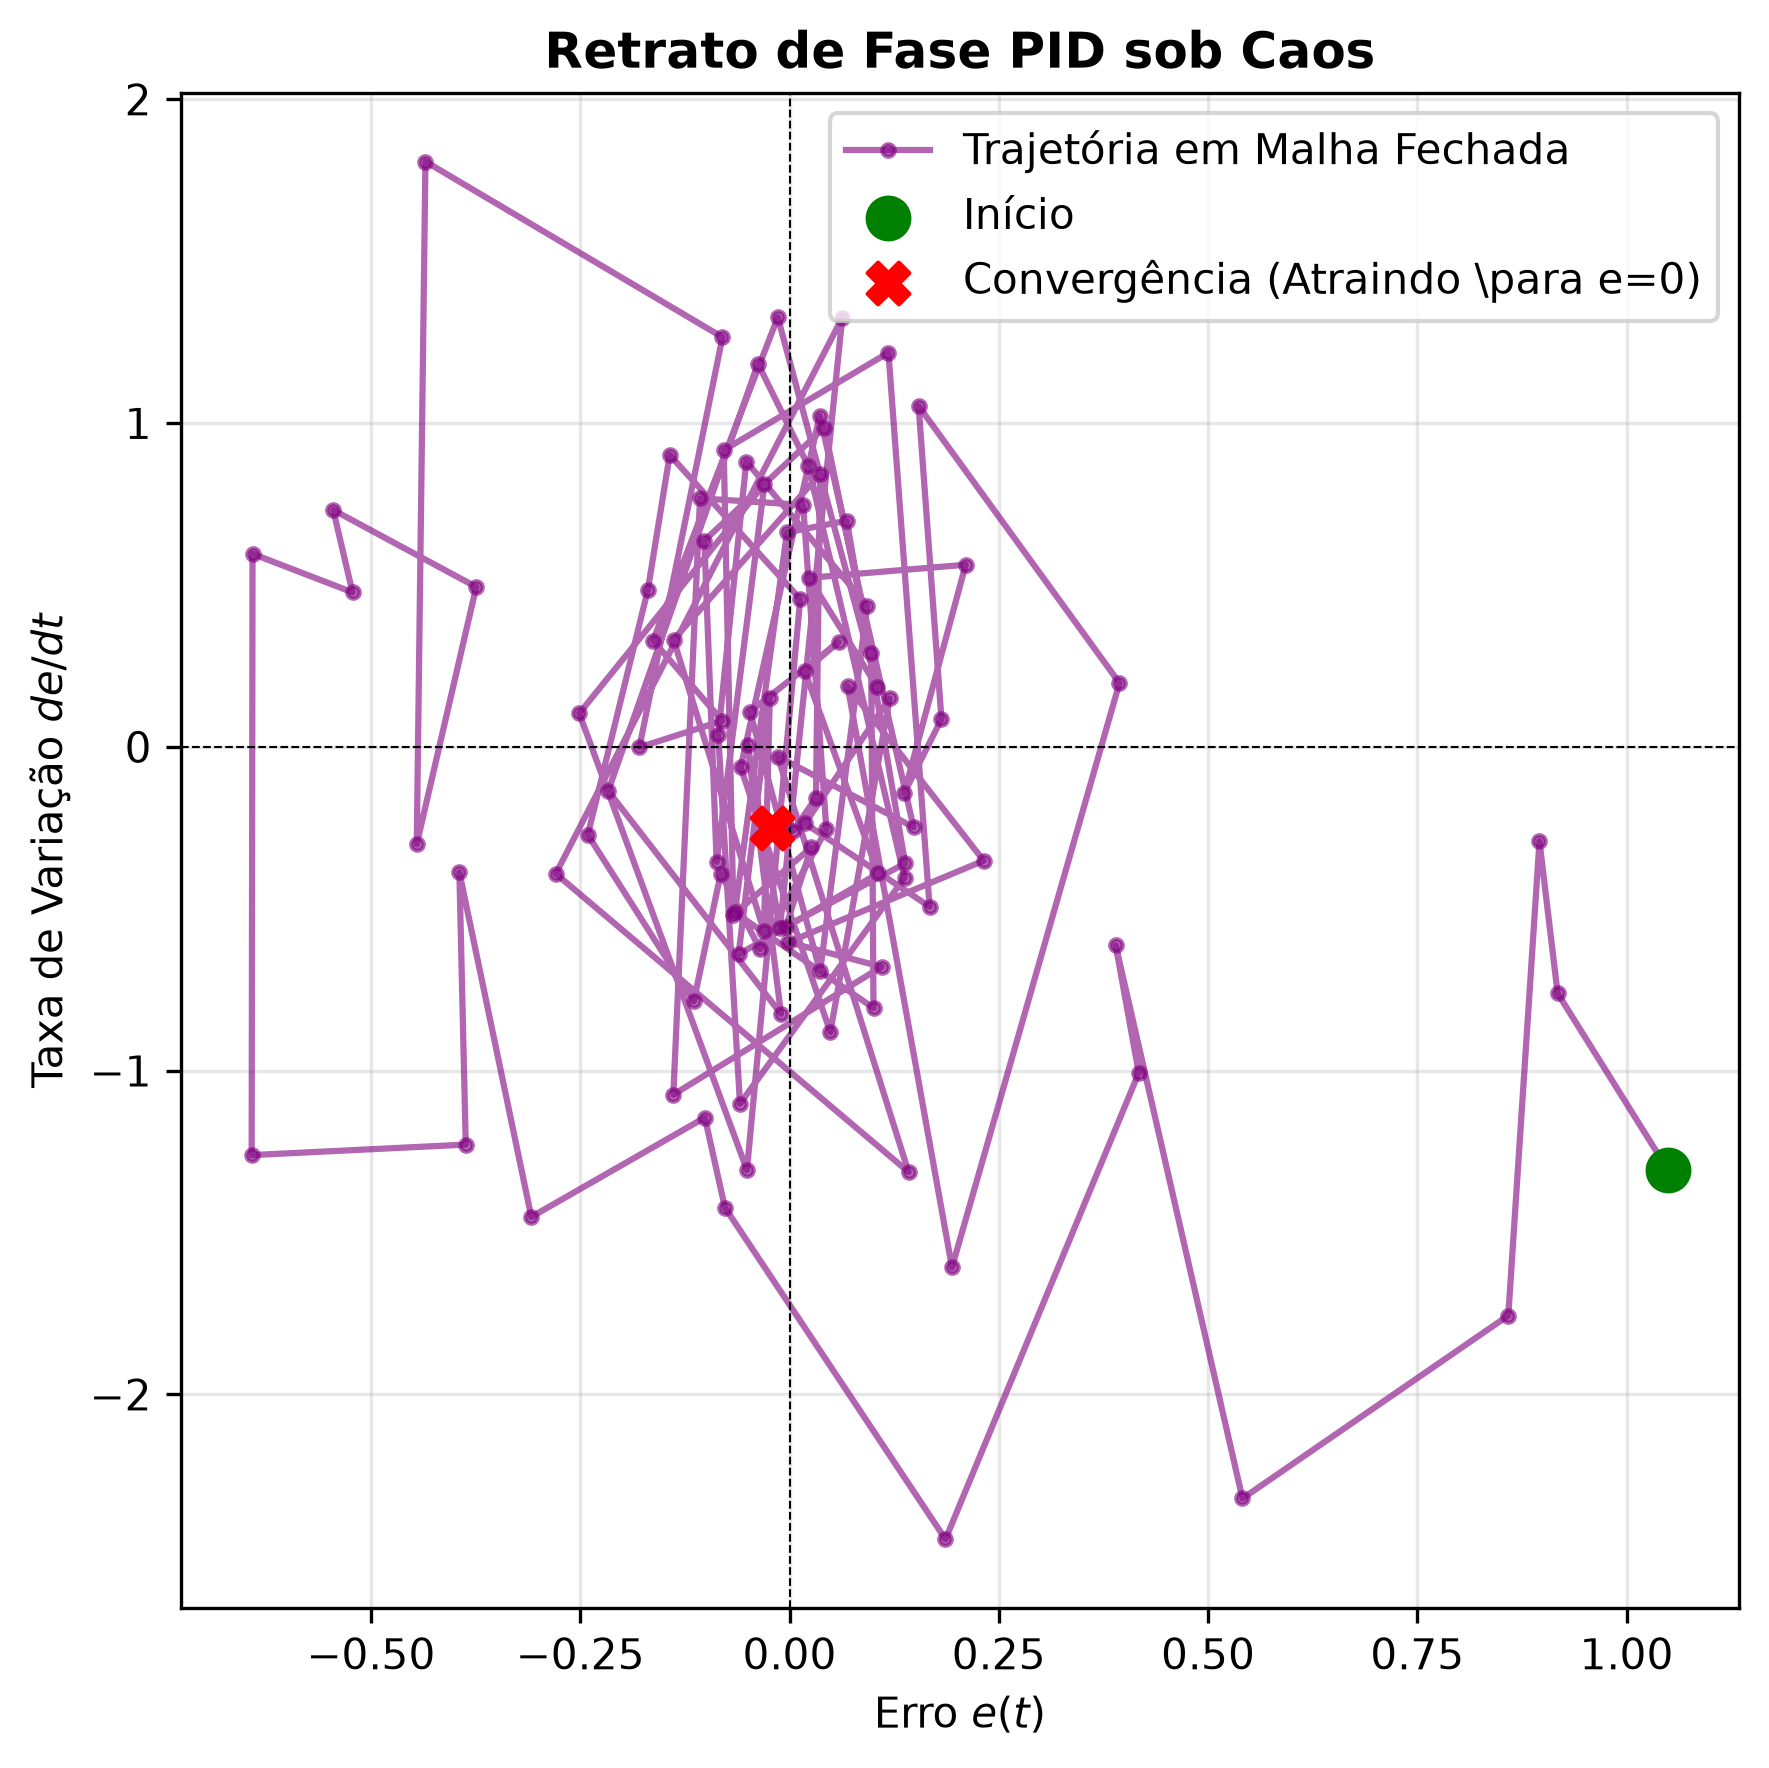
\includegraphics[width=0.80\textwidth]{plot_pid_phase_portrait.png}
\caption{Retrato de fase do controlador PID sob perturbação.}
\label{fig:fase}
\legend{\small Fonte: elaborada pelo autor, com semente fixa.}
\end{figure}

O erro de rastreamento diminui nos cinco perfis simulados, mas essa observação é finita e
\textbf{não} comprova estabilidade assintótica. A prova formal cobre exatamente
$T < 150\,^\circ$C, por dez passos, sob ruído de sensor em $[-5,+5]$; perturbações no atuador
não foram modeladas.

Este caso produziu o episódio metodologicamente mais instrutivo do ciclo. Uma primeira
medição, com limite de 200\,s, resultou em \textit{timeout}, e a afirmação esteve a ponto de
ser classificada como não sustentada por evidência. Reexecutada com folga, a mesma
propriedade foi \textbf{provada} --- pouco além do limite anterior. A lição é simétrica e vale
para todo o relatório: ler \textit{timeout} como ``seguro'' inventa uma prova; lê-lo como
``propriedade falsa'' descarta uma prova legítima. Nos dois casos o defeito é o mesmo, tratar
\emph{ausência de sinal como sinal}. É por isso que a coluna de veredito do arquivo de
evidências mantém \veredito{timeout} separado de \SAFE{} e de \UNSAFE{}, e nunca os colapsa.

\subsubsection{Biblioteca de controle de terceiros}

Para avaliar a aplicabilidade da abordagem a código de produção, a
\textit{Arduino-PID-Library} foi integrada como submódulo e submetida ao mesmo modelo de
planta e de ruído. \textbf{A verificação não foi concluída.} Foram encontrados três
obstáculos independentes, dois deles removidos:

\begin{enumerate}[leftmargin=1.4cm]
  \item o \textit{harness} declarava \texttt{void \_\_ESBMC\_assume(int)}, em conflito com a
  declaração \texttt{bool} dos \textit{intrinsics} do verificador, e por isso sequer era
  analisado --- \textbf{corrigido};
  \item a macro \texttt{ARDUINO} não era definida, fazendo o código recair em um ramo anterior
  ao Arduino 1.0 que requer um cabeçalho inexistente --- contornável por
  \texttt{-DARDUINO=100};
  \item \textbf{bloqueio remanescente}: o arquivo emprega \textbf{construtor delegante},
  recurso de C++11, e o ESBMC 6.8.0 não oferece a opção \texttt{--std}, introduzida apenas na
  8.0.0. O \textit{harness} usa justamente o construtor de sete argumentos, que é o delegante,
  de modo que o recurso não pode ser evitado.
\end{enumerate}

O registro relevante é que a barreira \textbf{não está} na complexidade do algoritmo de
controle, mas na cobertura do \textit{frontend} C++ do verificador e nas convenções de
compilação do ecossistema alvo. O mesmo defeito de declaração do primeiro item foi encontrado
e corrigido em outros dois arquivos do projeto, entre eles o \textit{stub} de bloco MLP, que
passou a ser verificável e figura como provado na Tabela~\ref{tab:evidencias}.

\subsection{Caso 5 --- blocos \textit{feed-forward} de modelos de linguagem}

A Tabela~\ref{tab:ffn} apresenta os tempos medidos do Método 2 --- ativação abstraída por
intervalos --- sobre blocos FFN extraídos do GPT-2 e do LLaMA-7B.

\begin{table}[H]
\centering
\caption{Verificação de blocos FFN com sobreaproximação intervalar da ativação (Método 2).}
\label{tab:ffn}
\small
\begin{tabular}{@{}llcrl@{}}
\toprule
\textbf{\textit{Harness}} & \textbf{Dimensões} & \textbf{Ativação} & \textbf{Tempo} &
\textbf{Veredito} \\
\midrule
\texttt{gpt2\_2x4\_qnn}     & $2{\times}4{\times}2$  & intervalo GeLU & 0,24\,s  & \SAFE \\
\texttt{llama-7b\_4x8\_qnn} & $4{\times}8{\times}4$  & intervalo SiLU & 3,46\,s  & \SAFE \\
\texttt{gpt2\_4x8\_qnn}     & $4{\times}8{\times}4$  & intervalo GeLU & 4,24\,s  & \SAFE \\
\texttt{gpt2\_4x16\_qnn}    & $4{\times}16{\times}4$ & intervalo GeLU & 20,10\,s & \SAFE \\
\bottomrule
\end{tabular}
\legend{\small Fonte: \texttt{results/EVIDENCIAS.md}; ESBMC 6.8.0 com Boolector.}
\end{table}

O crescimento entre $4{\times}8$ e $4{\times}16$ --- de 4,24\,s para 20,10\,s ao dobrar a
dimensão oculta --- é coerente com a barreira observada no Caso 2 e delimita o alcance
prático da técnica: a verificação é modular, aplicada a fatias representativas, e não ao
modelo completo. Um bloco de produção com $d = 4096$ geraria da ordem de $16$ milhões de
multiplicações simbólicas.

O ponto conceitual mais importante deste caso é o compromisso entre as duas codificações. O
Método 1, mais rápido, substitui a ativação por um \textit{proxy} ReLU e portanto verifica um
modelo \emph{que não é o modelo implantado}. O Método 2 verifica a propriedade sobre uma
relaxação intervalar, e a solidez do veredito para a ativação real depende inteiramente de os
limites injetados serem conservadores. Nenhuma das duas codificações é ``a correta'': a
codificação mais rápida não é a mais sólida, e essa tensão precisa ser declarada junto do
resultado.

Registre-se ainda que a documentação do subprojeto reporta um ganho de 18 a 27 vezes do
Método 2 otimizado sobre uma codificação inicial que usava Z3, inteiros de 64 bits e mantinha
código morto de pré-ativação. Essa razão \textbf{não} foi remedida neste trabalho; apenas os
tempos da Tabela~\ref{tab:ffn} o foram, e ficaram sistematicamente abaixo dos documentados
--- 4,24\,s contra 5,3\,s, 3,46\,s contra 4,3\,s, 20,10\,s contra 27\,s ---, diferença
compatível com variação de máquina.

\subsection{Caso 6 --- política de aprendizado por reforço}

O \textit{solver} encontrou \textbf{contraexemplo} em 2,58\,s: existe estado, dentro da caixa
analisada, para o qual a ação da política ultrapassa o intervalo $[-1,1]$ do atuador. A
Figura~\ref{fig:shield} apresenta a avaliação da mesma expressão do \textit{harness} sobre a
mesma caixa de estados, na qual a violação é visível --- a ação máxima atinge 1,50 contra o
limite de 1,0, e uma fração não desprezível da grade viola o limite.

\begin{figure}[H]
\centering
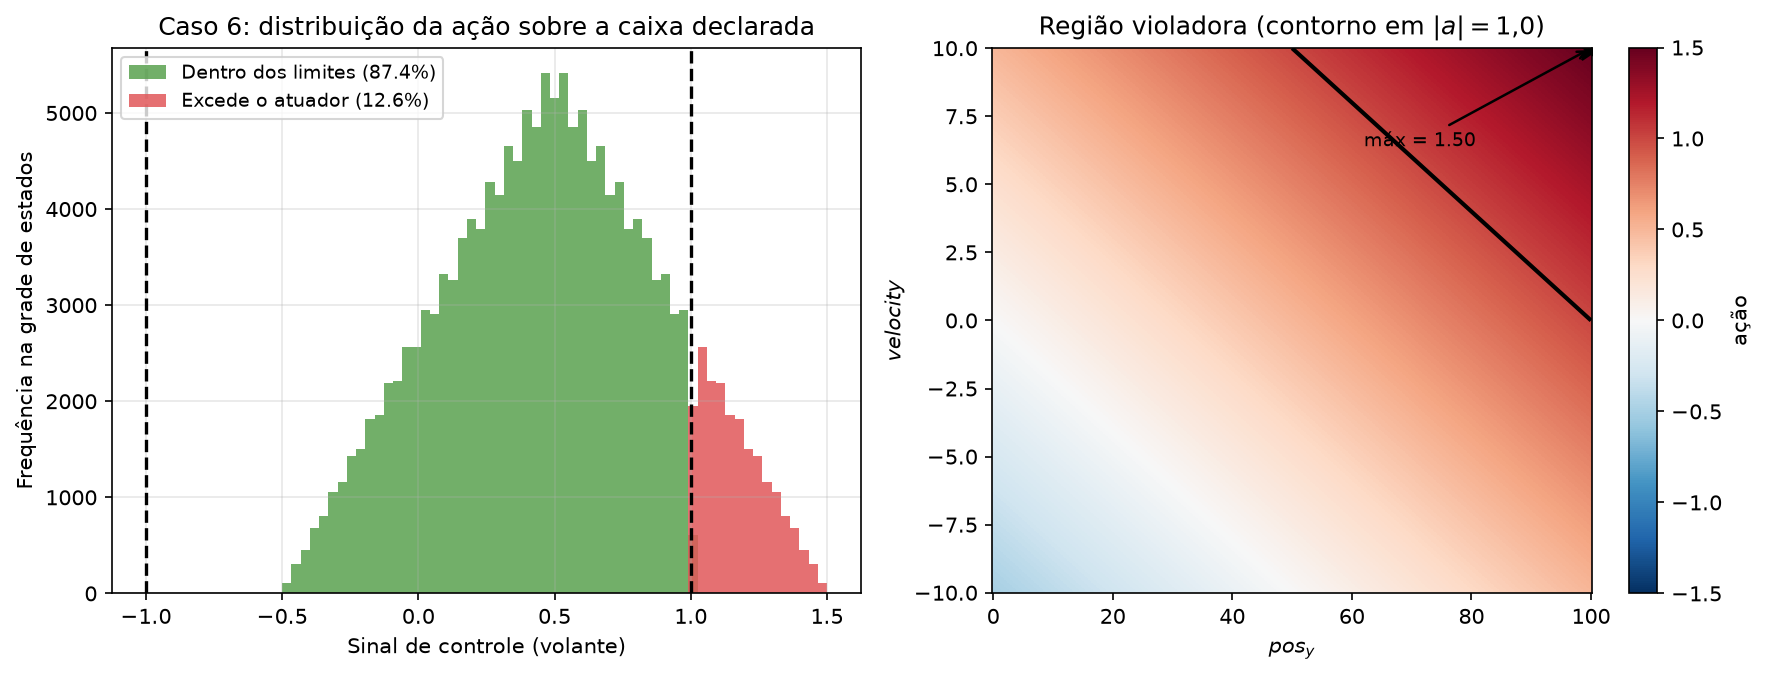
\includegraphics[width=0.86\textwidth]{plot_rl_shield.png}
\caption{Distribuição das ações da política sobre a caixa de estados do \textit{harness}: a
região que excede o limite do atuador é atingível.}
\label{fig:shield}
\legend{\small Fonte: elaborada pelo autor, avaliando a expressão do próprio
\textit{harness}.}
\end{figure}

A conclusão precisa ser enunciada com cuidado, porque é fácil invertê-la. O \textit{harness}
\textbf{detecta} a violação; ele \textbf{não} demonstra que o \textit{safety shield} a impeça.
O escudo precisa ser corrigido e novamente verificado antes de qualquer afirmação de proteção
pré-implantação. Reportar esse resultado negativo é preferível a apresentá-lo como validação
do escudo.

\subsection{Caso 7 --- malha fechada com controlador DDPG quantizado}
\label{sub:cartpole}

\subsubsection{Fidelidade da quantização}

As três implementações da inferência --- Python, TypeScript e C --- coincidem bit a bit. A
caracterização do erro de quantização sobre $10^4$ amostras, com escala 256 e força em
$[-10, +10]$\,N, dá erro absoluto médio de $0{,}078$\,N e percentil 95 de $0{,}226$\,N, com
erro absoluto máximo de $7{,}76$\,N. A cauda é relevante e está reportada: o erro típico é
pequeno, mas o pior caso não é desprezível, e é precisamente o pior caso que a verificação
formal explora.

\subsubsection{Duas propriedades vácuas}

O teste de vacuidade descrito na Seção~\ref{sub:vacuidade} revelou que duas das três
propriedades originalmente verificadas \textbf{não dependiam do controlador}:

\begin{itemize}[leftmargin=1.4cm]
  \item a propriedade de segurança em um passo asseria sobre
  $\theta_{\text{novo}} = \theta + 5\dot{\theta}/256$, expressão que não contém a força $F$.
  Executando a mesma asserção sem rede alguma e com $F$ arbitrária, veredito e contraexemplo
  se reproduzem idênticos: os 745 pesos eram \textbf{código morto} para aquela propriedade;
  \item a propriedade de limite de força, $|F| \le 10$\,N, vale por \textbf{construção} da
  aproximação de $\tanh$, que satura em Q8.8. Substituindo a rede inteira por uma entrada
  livre, a prova passa em 0,72\,s.
\end{itemize}

A correção seguiu dois caminhos distintos. A primeira propriedade foi reescrita para
\textbf{dois passos}, pois a força só alcança $\theta$ através de $\dot{\theta}$ no passo
seguinte; a dependência foi confirmada observando que o contraexemplo muda conforme $F$ é
livre ou nula. A segunda foi \textbf{reclassificada} como verificação de sanidade da
quantização --- ela detecta erro de tabela ou de escala, o que é útil, mas não é prova sobre o
ator --- e uma propriedade nova foi introduzida para cobrir o que ela não podia decidir: na
zona de perigo, o controlador deve aplicar força de magnitude mínima, condição que um
controlador inerte viola e cuja decisão exige percorrer os pesos. A discriminação foi
verificada nos dois sentidos: a nova propriedade falha para um controlador nulo e é provada
para um controlador atuante.

Esta é a contribuição metodológica que o projeto considera mais transferível. Uma propriedade
vácua não produz erro, não produz aviso e não produz número implausível: produz uma prova
verdadeira sobre o objeto errado. O único mecanismo que a expõe é o teste explícito de
dependência.

\subsubsection{Envelope de segurança e a barreira do BMC}

A Tabela~\ref{tab:envelope} caracteriza a propriedade corrigida de dois passos em função da
velocidade angular inicial admitida.

\begin{table}[H]
\centering
\caption{Segurança em dois passos em função do limite admitido de $|\dot{\theta}|$.}
\label{tab:envelope}
\small
\begin{tabular}{@{}rrlr@{}}
\toprule
$|\dot{\theta}| \le$ (Q8.8) & \textbf{rad/s} & \textbf{Veredito} & \textbf{Tempo} \\
\midrule
1280 & 5,00 & \UNSAFE   & 25,4\,s \\
 640 & 2,50 & \UNSAFE   & 28,8\,s \\
 320 & 1,25 & Indeciso  & $>$\,300\,s \\
 160 & 0,62 & Indeciso  & $>$\,300\,s \\
  80 & 0,31 & Indeciso  & $>$\,300\,s \\
\bottomrule
\end{tabular}
\legend{\small Fonte: elaborada pelo autor; limite de 300\,s por instância.}
\end{table}

O resultado defensável é, portanto: a segurança de dois passos é \textbf{violada} acima de
2,5\,rad/s e \textbf{indecisa} abaixo disso. \textbf{Não} se conclui que o controlador seja
seguro em nenhuma faixa.

O comportamento da tabela contraria a intuição e merece explicação, porque \textbf{reduzir a
região inicial torna o problema mais difícil}. Com uma caixa ampla existe contraexemplo, e
encontrá-lo é a direção barata do problema: basta ao \textit{solver} exibir uma testemunha.
Nas caixas estreitas não há testemunha a exibir, e decidir exige \emph{provar} a ausência de
violação --- a direção cara. A assimetria entre satisfatibilidade e insatisfatibilidade é,
aqui, o fator dominante do custo.

A verificação de malha fechada obtida neste trabalho é de horizonte curto. Um
\textit{harness} de cinquenta passos chegou a ser esboçado e nunca foi concluído, e a leitura
imediata seria falta de tempo. A medição mostra outra coisa: para a rede sintética, o custo de
provar $K$ passos cresce de 0,3\,s e 46\,MB em $K{=}1$ para \textbf{909\,s e 383\,MB} em
$K{=}4$. A barreira não está em cinquenta passos; está em quatro. É limite do método, não do
esforço.

\subsubsection{\textit{Model checking} indutivo como alternativa}

A causa da barreira é estrutural: o BMC constrói \emph{uma} fórmula contendo $K$ cópias da
relação de transição. O IC3/PDR nunca constrói essa fórmula, e seu resultado é um invariante
indutivo --- ``seguro sempre'' em vez de ``seguro até $K$''.

O sistema acoplado foi exportado como sistema de transição em Verilog e sintetizado pelo
Yosys, resultando em \textbf{904.242 portas AND, 65 registradores e nível lógico 689}. A
propriedade verificada é $|\theta| \le 53$ em Q8.8, equivalente a aproximadamente
$12^\circ$, a partir de uma caixa inicial de estados. A validação diferencial do Verilog
gerado contra a referência coincidiu em 12 de 12 estados amostrados --- o que detecta
regressão de tradução, mas não prova equivalência universal. A Tabela~\ref{tab:ic3} reúne os
resultados.

\begin{table}[H]
\centering
\caption{\textit{Bounded model checking} contra \textit{model checking} indutivo.}
\label{tab:ic3}
\small
\begin{tabular}{@{}lllrr@{}}
\toprule
\textbf{Método} & \textbf{Modelo} & \textbf{Veredito} & \textbf{Tempo} & \textbf{Memória} \\
\midrule
BMC (ESBMC) & sintético, $K{=}4$        & seguro até 4 passos           & 909\,s  & 383\,MB \\
IC3 (ABC)   & sintético com batente     & \textbf{provado $\forall t$}  & 0,37\,s & trivial \\
IC3 (ABC)   & ator DDPG real            & não convergiu                 & 1802\,s & 708\,MB \\
BMC (ABC)   & ator DDPG real            & 5 \textit{frames}, sem veredito & 901\,s & 503\,MB \\
\bottomrule
\end{tabular}
\legend{\small Fonte: \texttt{ic3/EVIDENCIA.md}. \textit{Timeout} é indeciso, não ``seguro''.}
\end{table}

No modelo sintético com batente mecânico, o IC3 produziu prova ilimitada em 0,37\,s, com um
invariante de quatro cláusulas sobre \textbf{três dos 65 bits de estado}: o algoritmo
determinou por conta própria que os bits altos de $\theta$ permanecem iguais ao sinal e que as
mais de cem mil portas da rede são irrelevantes para a prova. Nenhuma execução de BMC produz
esse tipo de resultado, e a diferença de três ordens de grandeza no tempo não é a parte mais
importante: a parte mais importante é que o veredito é \emph{ilimitado}.

Sobre o controlador real, contudo, \textbf{nenhum dos dois métodos decide}. O PDR foi
interrompido em 1802\,s sem convergir e o BMC alcançou cinco \textit{frames} em 901\,s. É um
empate técnico, e é assim que deve ser reportado --- \textit{timeout} é indeciso, e tratá-lo
como ``seguro'' seria repetir exatamente o erro que este projeto passou o ciclo corrigindo.

Registre-se uma lacuna de evidência nesta medição: a saída bruta daquela execução de PDR
\textbf{não foi preservada}, porque o \textit{script} então filtrava a saída por
palavras-chave antes de gravá-la. Restam tempo e pico de memória, medidos pelo invólucro. O
defeito foi corrigido --- a saída bruta passou a ser sempre salva ---, mas a medição histórica
permanece qualificada como tal em vez de ser apresentada como plenamente reproduzível.

A semelhança entre as duas barreiras --- cinco \textit{frames} no ator real de 745 parâmetros
e $K{=}4$ na rede sintética, cerca de oito vezes menor --- é sugestiva de um limite de
escalabilidade, mas modelos, propriedades, representações e \textit{solvers} diferem entre as
duas medições. Elas motivam uma hipótese; não isolam causalidade nem demonstram que o limite
pertença ao método.

A hipótese remanescente é de \textbf{representação}. A tradução para AIGER converte quatro
palavras de estado em 65 bits isolados, dissolvendo exatamente a estrutura sobre a qual o PDR
generaliza cláusulas: o invariante precisaria falar sobre $\theta$ \emph{como palavra}, e não
sobre bits soltos. Atacar essa hipótese exige exportar o sistema em BTOR2, que preserva as
palavras, e empregar um motor de nível de palavra. Essa é a continuidade direta indicada na
Seção~\ref{sec:conclusao}, e é uma mudança de \emph{representação}, não de motor.

\subsection{Síntese comparativa}

A Tabela~\ref{tab:sintese} organiza os sete casos segundo o que efetivamente foi estabelecido
e o que permanece em aberto.

\begin{table}[H]
\centering
\caption{Síntese dos sete estudos de caso: o que foi estabelecido e sob quais condições.}
\label{tab:sintese}
\footnotesize
\begin{tabular}{@{}p{1.5cm}p{4.4cm}p{4.0cm}p{3.6cm}@{}}
\toprule
\textbf{Caso} & \textbf{O que foi estabelecido} & \textbf{Sob quais hipóteses} &
\textbf{Em aberto} \\
\midrule
1 & Rede quantizada provada; propriedade sobre a rede em ponto flutuante violada &
Domínio discreto (XOR); intervalos por neurônio injetados &
Verificação a partir do modelo em Python \\
\addlinespace
2 & Contraexemplo de memória; GEMM provado até $N{=}3$ &
$\texttt{seq\_len} \in [1,10]$; limite de 300\,s &
Dimensões de produção \\
\addlinespace
3 & Protocolo gerar--verificar--corrigir demonstrado em 2 iterações &
Gerador \textit{mock} determinístico; \texttt{--unwind 32} &
Agente de linguagem real \\
\addlinespace
4 & $T < 150\,^\circ$C provado por 10 passos &
Ruído de sensor em $[-5,+5]$; sem perturbação de atuador &
Estabilidade assintótica; biblioteca C++11 \\
\addlinespace
5 & Quatro blocos FFN provados, até $4{\times}16$ &
Sobreaproximação intervalar da ativação &
Solidez para a ativação real; escala $d{=}4096$ \\
\addlinespace
6 & Contraexemplo: a ação excede o limite do atuador &
Caixa de estados do \textit{harness} &
\textit{Safety shield} corrigido e verificado \\
\addlinespace
7 & Vacuidades corrigidas; violação acima de 2,5\,rad/s; barreira do BMC medida &
Horizonte de dois passos; quantização Q8.8 &
Faixas baixas indecisas; representação word-level \\
\bottomrule
\end{tabular}
\legend{\small Fonte: elaborada pelo autor.}
\end{table}

Lida em conjunto, a tabela sugere uma regularidade que o projeto considera seu achado central.
A verificação formal de componentes de IA é \textbf{praticável e informativa em escala
modular}: blocos, \textit{kernels} e redes pequenas são decididos em segundos, e os
contraexemplos obtidos são acionáveis. O acoplamento com a planta, por outro lado, esbarra em
uma barreira que não é de implementação nem de esforço, e que se manifesta em horizontes de
poucos passos. Entre esses dois regimes está o espaço em que o método rende mais: propriedades
locais, hipóteses declaradas explicitamente e vereditos qualificados pelo horizonte.

% =====================================================================
\section{Limitações, ameaças à validade e dificuldades encontradas}
\label{sec:limitacoes}

\subsection{Limitações do que foi provado}

As garantias obtidas neste trabalho são condicionais, e a lista abaixo delimita exatamente a
que condições:

\begin{itemize}[leftmargin=1.4cm]
  \item \textbf{Horizonte finito.} Todos os vereditos de BMC valem até o limite de
  desenrolamento indicado. A verificação em malha fechada cobre dois passos; o
  \textit{harness} de cinquenta passos não foi concluído e a medição mostra que o custo
  torna-o inviável nesta máquina.
  \item \textbf{Indecisão sob faixas estreitas.} Abaixo de 1,25\,rad/s, a propriedade de dois
  passos permanece indecisa em 300\,s. Não há, portanto, faixa de operação em que o
  controlador esteja provado seguro.
  \item \textbf{Nenhum dos dois métodos decide o controlador real.} O PDR não convergiu em
  1802\,s e o BMC alcançou cinco \textit{frames} em 901\,s.
  \item \textbf{Sobreaproximação nas ativações.} Os quatro vereditos de blocos FFN valem para
  a relaxação intervalar injetada. Transferi-los para GeLU e SiLU reais exige que esses
  limites sejam conservadores, o que não foi provado --- o \textit{encoding} não representa a
  relação funcional exata.
  \item \textbf{Aproximação linear da sigmoide.} Onde a forma funcional foi mantida, a
  substituição por $\operatorname{clip}(0{,}25z + 0{,}5, 0, 1)$ altera a função implantada; o
  veredito vale para a aproximação.
  \item \textbf{Perfis de caos com faixa contínua não decidem} sob \texttt{--floatbv}; apenas
  o perfil discreto de impulso decide, em 27\,s.
  \item \textbf{Verificação a partir de Python não realizada.} O binário disponível não possui
  o \textit{frontend} Python compilado.
  \item \textbf{Biblioteca de terceiros não verificada.} O bloqueio é a ausência de
  \texttt{--std} na versão 6.8.0, necessária para o construtor delegante de C++11.
\end{itemize}

\subsection{Ameaças à validade}

\subsubsection{Validade de construção: a propriedade vácua}

A ameaça mais séria identificada no ciclo não é de desempenho, mas de significado. Uma
propriedade que decide sem envolver o artefato produz uma prova verdadeira sobre um objeto
que não interessa, e não emite nenhum sinal de erro. Duas das três propriedades da malha
fechada estavam nessa condição, e foram descobertas apenas pelo teste explícito de
dependência descrito na Seção~\ref{sub:vacuidade}. Não há razão para supor que o repositório
esteja hoje livre de casos análogos; o que existe é um procedimento para detectá-los, e ele
deve ser aplicado a toda propriedade nova.

\subsubsection{Validade interna: fidelidade das traduções}

Três traduções sustentam os resultados e nenhuma delas está provada correta. A quantização
Q8.8 do ator coincide bit a bit entre três implementações, o que é evidência forte de
consistência interna, mas não de fidelidade ao modelo treinado em ponto flutuante --- a
caracterização de erro mostra pior caso de 7,76\,N. A tradução para Verilog foi validada por
teste diferencial em doze estados: isso detecta regressão, não equivalência. E os
\textit{stubs} de blocos de \textit{transformer} representam fatias reduzidas, não os módulos
de produção.

\subsubsection{Validade externa: escala e generalização}

Os experimentos foram conduzidos em uma única máquina de quatro núcleos, com um binário
específico do verificador. As barreiras medidas --- $N{=}4$ no GEMM, $K{=}4$ na malha fechada,
cinco \textit{frames} no ABC --- são propriedades daquele ambiente e daqueles
\textit{harnesses}, e não constantes do método. Extrapolá-las seria repetir o defeito que a
auditoria do projeto encontrou e corrigiu.

\subsubsection{Validade de conclusão: procedência dos números}

Este relatório reporta apenas números com log bruto versionado, com uma exceção declarada: a
execução histórica de PDR sobre o ator real, cuja saída bruta se perdeu antes da correção do
\textit{script}. Ela é apresentada como medição histórica do invólucro, e não como resultado
plenamente reproduzível.

\subsection{Dificuldades encontradas ao longo do ciclo}

Registram-se as dificuldades que mais consumiram tempo, na expectativa de que sejam úteis a
quem retomar o trabalho:

\begin{enumerate}[leftmargin=1.4cm]
  \item \textbf{Defeitos silenciosos na instrumentação.} Vários experimentos produziam números
  plausíveis sem medir nada: um parâmetro de dimensão que não chegava ao código compilado, uma
  \textit{flag} que fazia o verificador emitir a fórmula em vez de resolvê-la, um portão de
  verificação comentado em um orquestrador. Nenhum deles emitia erro. Foram encontrados apenas
  por auditoria dirigida, e não por execução da suíte.
  \item \textbf{Suíte de testes verde sem verificar.} A suíte chegou a passar sem exercitar o
  verificador, porque o resultado era reduzido a um booleano que também é falso quando nada
  executa. A reescrita do invólucro e a suíte de regressão de casos-limite foram respostas
  diretas a isso.
  \item \textbf{Divergência entre binário e árvore de código.} O binário versionado é a versão
  6.8.0 e a árvore presente no repositório é a 8.0.0, não compilada. \textit{Flags} da 8.0.0
  são rejeitadas pela 6.8.0 com código 64, facilmente confundível com propriedade violada.
  Compilar a 8.0.0 leva de uma a quatro horas, o que tornou a alternância custosa.
  \item \textbf{Escolha de limites de tempo.} O episódio do PID mostra o custo de um limite
  arbitrário: 200\,s produziram \textit{timeout} para uma propriedade que é verdadeira e se
  prova em pouco mais que isso.
  \item \textbf{Submódulo Git inconsistente.} Um \textit{gitlink} sem entrada correspondente em
  \texttt{.gitmodules} fazia o \textit{checkout} automatizado terminar com erro. O conteúdo foi
  recuperado --- e não descartado --- após identificar o repositório e o \textit{commit}
  corretos.
  \item \textbf{Peso do repositório.} Material de terceiros vendorizado responde por
  308\,MB dos 322\,MB do diretório do projeto, o que penaliza clonagem e integração contínua.
  A decisão sobre o que preservar permanece em aberto.
\end{enumerate}

% =====================================================================
\section{Conclusões}
\label{sec:conclusao}

Este relatório apresentou a aplicação de \textit{bounded model checking} baseado em SMT, por
meio do verificador ESBMC, a sete classes de artefatos de inteligência artificial, do neurônio
quantizado isolado à malha fechada formada por planta \textit{cart-pole} e controlador DDPG.
Dos doze \textit{harnesses} reexecutáveis consolidados, nove foram provados, três produziram
contraexemplo e nenhum ficou indeciso, todos com saída bruta do \textit{solver} versionada.

Quatro conclusões se sustentam sobre a evidência apresentada.

\textbf{Primeira: a verificação formal de componentes de IA é praticável em escala modular e
produz informação que a amostragem não produz.} O caso mais eloquente é o do Caso 1, em que
$10^4$ amostras não exibem violação alguma e o \textit{solver} encontra, em 197\,s, uma
entrada admissível que excede o limite declarado. Contraexemplos são acionáveis: no ciclo
neuro-simbólico, o diagnóstico com deslocamento exato da violação fecha o ciclo de correção em
uma iteração.

\textbf{Segunda: a maior ameaça a este tipo de trabalho é a propriedade vácua, e ela não emite
sinal.} Duas das três propriedades da malha fechada decidiam sem que os 745 parâmetros do
controlador participassem da prova. Elas não produziam erro, aviso ou número implausível ---
produziam provas verdadeiras sobre o objeto errado. O único mecanismo que as expôs foi o teste
explícito de dependência: remover o modelo e verificar se o veredito muda. Esse teste é barato
e deveria ser rotina em qualquer verificação de rede neural.

\textbf{Terceira: a barreira do BMC em malha fechada é do método, não do esforço, e foi
medida.} Provar $K$ passos custa 0,3\,s em $K{=}1$ e 909\,s em $K{=}4$, com memória crescendo
de 46\,MB para 383\,MB. O \textit{harness} de cinquenta passos não ficou por fazer: ele é
inviável nesta máquina. Reconhecer isso transforma a maior limitação do trabalho em resultado,
desde que a comparação seja feita com honestidade.

\textbf{Quarta: o \textit{model checking} indutivo é a direção certa, mas a instância real
exige atacar a representação, e não trocar de motor.} No modelo sintético, o IC3 produziu
prova \emph{ilimitada} em 0,37\,s, com invariante de quatro cláusulas sobre três dos 65 bits
de estado, onde o BMC levou 909\,s para quatro passos. Sobre o controlador real, entretanto,
nenhum dos dois métodos decide: o PDR não convergiu em 1802\,s e o BMC parou em cinco
\textit{frames} em 901\,s. A hipótese mais plausível para esse impasse é a perda de estrutura
na tradução: converter quatro palavras de estado em 65 bits isolados destrói exatamente aquilo
sobre o que o PDR generaliza cláusulas.

Além dos vereditos, o ciclo entrega uma infraestrutura de reprodutibilidade que é, em si, um
resultado: um invólucro que distingue erro de execução de propriedade violada, uma suíte de
regressão que congela essa distinção, um gerador que reexecuta cada afirmação do texto e
versiona a saída bruta, e um índice que liga cada número deste relatório ao log que o produziu.

\subsection{Perspectivas de continuidade}

Cinco direções decorrem diretamente do que foi medido, em ordem de prioridade:

\begin{enumerate}[leftmargin=1.4cm]
  \item \textbf{Representação em nível de palavra.} Exportar o sistema de transição em BTOR2,
  que preserva as quatro palavras de estado em vez de dissolvê-las em bits, e empregar um motor
  word-level. É a continuidade direta do impasse do Caso 7 e a hipótese que o projeto considera
  mais promissora.
  \item \textbf{Fechar a curva de escalabilidade do BMC} no modelo sintético, medindo $K{=}8$ e
  $K{=}16$, para caracterizar a barreira em vez de a supor. A medição deve permanecer no modelo
  sintético: no modelo real, cinco \textit{frames} em 901\,s já indicam que esses horizontes
  estão fora de alcance nesta máquina.
  \item \textbf{Corrigir e verificar o \textit{safety shield}} do Caso 6, de modo que o
  contraexemplo hoje obtido deixe de ser atingível, e reverificar a propriedade sobre o escudo
  corrigido.
  \item \textbf{Compilar o ESBMC 8.0.0} com o \textit{frontend} Python habilitado, o que
  desbloqueia simultaneamente a verificação a partir de modelos em Python e a da biblioteca de
  controle em C++11 --- dois objetivos hoje impedidos pelo mesmo obstáculo.
  \item \textbf{Substituir a sobreaproximação intervalar} das ativações por limites derivados
  de propagação de intervalos sobre os pesos reais, tornando o conservadorismo verificável em
  vez de assumido, e manter o teste de vacuidade das hipóteses como guarda permanente.
\end{enumerate}

Encerra-se com a observação metodológica que atravessou todo o ciclo. O erro que mais
frequentemente compromete trabalhos desta natureza não é provar algo falso --- o
\textit{solver} raramente permite isso --- mas \textbf{tratar ausência de sinal como sinal}:
ler \textit{timeout} como segurança, ler suíte verde como verificação, ler número plausível
como medição. As correções mais importantes deste PIBIC foram todas dessa família, e a
infraestrutura construída existe para que elas não se repitam silenciosamente.

% =====================================================================
\section{Cronograma de atividades executadas}
\label{sec:cronograma}

A Tabela~\ref{tab:cronograma} apresenta a distribuição das atividades ao longo da vigência.
As marcações correspondem aos períodos de execução; os bimestres anteriores a fevereiro de
2026 antecedem o registro versionado do projeto e devem ser conferidos contra o plano de
trabalho aprovado antes da entrega \pendente{conferir os dois primeiros bimestres com o plano
aprovado}.

\begin{table}[H]
\centering
\caption{Cronograma executado, por bimestre da vigência 2025--2026.}
\label{tab:cronograma}
\footnotesize
\setlength{\tabcolsep}{4pt}
\begin{tabular}{@{}p{6.6cm}cccccc@{}}
\toprule
\multirow{2}{*}{\textbf{Atividade}} & \multicolumn{6}{c}{\textbf{Bimestre}} \\
\cmidrule(l){2-7}
 & 1º & 2º & 3º & 4º & 5º & 6º \\
\midrule
Revisão bibliográfica em verificação formal, BMC/SMT e verificação de redes neurais
 & X & X & X &   &   &   \\
Preparação do ambiente e do repositório; estudo do ESBMC e de suas primitivas
 & X & X &   &   &   &   \\
Caso 1 --- redes quantizadas e \textit{stubs} de inferência
 &   & X & X & X &   &   \\
Caso 2 --- \textit{kernels} de inferência e estudo de escalabilidade
 &   &   & X & X &   &   \\
Caso 3 --- ciclo neuro-simbólico de geração e correção
 &   &   & X & X &   &   \\
Caso 4 --- controlador PID sob ruído e biblioteca de terceiros
 &   &   &   & X & X &   \\
Caso 5 --- blocos \textit{feed-forward} de modelos de linguagem
 &   &   &   & X & X &   \\
Caso 6 --- política de aprendizado por reforço
 &   &   &   & X & X &   \\
Caso 7 --- malha fechada \textit{cart-pole} com controlador DDPG
 &   &   &   &   & X & X \\
Construção da camada \texttt{core\_verify} e da suíte de regressão
 &   &   &   &   & X & X \\
Auditoria de evidências, correção das propriedades vácuas e reexecução dos
\textit{harnesses}
 &   &   &   &   &   & X \\
Pipeline IC3/PDR: geração do sistema de transição, síntese e verificação indutiva
 &   &   &   &   &   & X \\
Redação do artigo, do relatório final e preparação da apresentação
 &   &   &   &   & X & X \\
\bottomrule
\end{tabular}
\legend{\small Fonte: elaborada pelo autor.}
\end{table}

\subsection{Produtos gerados}

A Tabela~\ref{tab:produtos} relaciona os produtos entregues ao artefato correspondente no
repositório, de modo que cada item seja verificável de forma independente.

\begin{table}[H]
\centering
\caption{Produtos do ciclo e respectivos artefatos de verificação.}
\label{tab:produtos}
\footnotesize
\begin{tabular}{@{}p{6.0cm}p{8.0cm}@{}}
\toprule
\textbf{Produto} & \textbf{Artefato} \\
\midrule
Doze \textit{harnesses} de verificação reexecutáveis &
\texttt{scripts/gerar\_evidencias.py}, \texttt{results/logs/} \\
Tabela consolidada de evidências &
\texttt{results/EVIDENCIAS.md} \\
Invólucro programático com status tri-estado &
\texttt{core\_verify/esbmc\_caller.py} \\
Analisador de contraexemplos &
\texttt{core\_verify/SMT\_feedback\_parser.py} \\
Suíte de regressão, incluindo os quatro modos de falha &
\texttt{tests/}, com destaque para \texttt{tests/test\_ground\_truth.py} \\
Propriedades corrigidas da malha fechada e caracterização do envelope &
\texttt{cartpole/verify\_ddpg\_closed\_loop.py},
\texttt{cartpole/caracteriza\_prop\_b.py} \\
Pipeline de verificação ilimitada por IC3/PDR &
\texttt{ic3/gen\_transition\_system.py}, \texttt{ic3/validate\_forward.py},
\texttt{ic3/run\_pdr.sh} \\
Evidência das medições indutivas &
\texttt{ic3/EVIDENCIA.md} \\
Geradores e tabelas de consulta dos blocos FFN &
\texttt{cases/llm\_ffn\_verification/} \\
Regeneração reprodutível das figuras &
\texttt{artigo/figs/gerar\_figuras.sh} \\
Documentação de uso e de limitações conhecidas &
\texttt{pibic/README.md}, \texttt{cartpole/ESBMC\_NOTES.md} \\
Backlog auditado com procedência de evidência por tarefa &
\texttt{KANBAN.md} \\
\bottomrule
\end{tabular}
\legend{\small Fonte: elaborada pelo autor.}
\end{table}

\subsection{Participação em eventos e produção associada}

\pendente{listar aqui apresentação no Congresso de Iniciação Científica da UFAM, resumos
submetidos, participação em eventos e eventuais publicações decorrentes do plano}


% --- referencias -----------------------------------------------------
\clearpage
\phantomsection
\addcontentsline{toc}{section}{REFERÊNCIAS}
\bibliographystyle{abntex2-alf}
\bibliography{referencias}

% --- apendices -------------------------------------------------------
\clearpage
% =====================================================================
\clearpage
\phantomsection
\section*{APÊNDICE A --- REPRODUTIBILIDADE}
\label{ap:reprodutibilidade}
\addcontentsline{toc}{section}{APÊNDICE A -- REPRODUTIBILIDADE}

\subsection*{A.1 Preparação do ambiente}

O binário do verificador acompanha o repositório, de modo que não há etapa obrigatória de
compilação para reproduzir os resultados reportados na Seção~\ref{sec:resultados}.

\begin{lstlisting}[language=bash]
git clone --recurse-submodules <url-do-repositorio>
cd esbmc/pibic
python3 -m venv .venv && source .venv/bin/activate
python -m pip install -e ".[test]"
pytest tests/ -v
\end{lstlisting}

O invólucro localiza o binário nesta ordem: a variável \texttt{\$ESBMC\_BIN}; \texttt{esbmc}
no \texttt{\$PATH}; uma compilação local em \texttt{../build/src/esbmc/esbmc}; e, por fim, o
binário versionado. Se nenhum existir, a suíte é \textbf{pulada} com motivo explícito, em vez
de acumular erros que seriam confundidos com falhas de propriedade.

\subsection*{A.2 Reexecução das evidências}

\begin{lstlisting}[language=bash]
python scripts/gerar_evidencias.py       # reexecuta os 12 harnesses
# saida bruta -> results/logs/*.log
# tabela      -> results/EVIDENCIAS.md
\end{lstlisting}

\subsection*{A.3 Verificação ilimitada por IC3/PDR}

\begin{lstlisting}[language=bash]
sudo apt-get install -y yosys            # traz o ABC embutido
cd ic3
python3 gen_transition_system.py --bits 16 -o cl_ddpg16.v
python3 validate_forward.py              # teste diferencial em 12 estados
./run_pdr.sh cl_ddpg16.v 1800
\end{lstlisting}

A execução de \texttt{validate\_forward.py} não é opcional: ela compara o Verilog gerado com
a referência em ponto fixo antes de qualquer medição. A coincidência das doze amostras detecta
regressão de tradução; não constitui prova de equivalência universal.

\subsection*{A.4 Compilação deste relatório}

\begin{lstlisting}[language=bash]
cd pibic/relatorio_final
make                 # pdflatex -> bibtex -> pdflatex -> pdflatex
make clean           # remove os intermediarios
\end{lstlisting}

As figuras são localizadas por \texttt{\textbackslash graphicspath} em \texttt{figuras/} e,
subsidiariamente, em \texttt{../artigo/figs/}. São necessários os pacotes
\texttt{texlive-latex-base}, \texttt{texlive-latex-recommended},
\texttt{texlive-latex-extra}, \texttt{texlive-fonts-recommended},
\texttt{texlive-lang-portuguese} e \texttt{texlive-publishers}, este último por fornecer
\texttt{abntex2cite} e o estilo bibliográfico \texttt{abntex2-alf}.

\subsection*{A.5 Advertências operacionais}

\begin{itemize}[leftmargin=1.4cm]
  \item \textbf{Nunca testar \texttt{not r.is\_safe} para concluir que um defeito foi
  encontrado.} Esse valor também é falso quando o verificador não executou. Use
  \texttt{r.status == UNSAFE}.
  \item \textbf{\texttt{--bounds-check} e \texttt{--pointer-check} não existem} no ESBMC:
  essas verificações são ativadas por padrão e a ferramenta expõe apenas as formas negativas,
  \texttt{--no-bounds-check} e \texttt{--no-pointer-check}. Passar as formas inexistentes
  encerra o processo com código 64.
  \item \textbf{\texttt{TIMEOUT} é indeciso}, nunca ``seguro''.
  \item \textbf{\texttt{--no-unwinding-assertions} só é seguro em \textit{harnesses} sem
  laços.} Em código com laços, o uso da opção pode tornar o caso vácuo.
\end{itemize}

% =====================================================================
\clearpage
\phantomsection
\section*{APÊNDICE B --- ÍNDICE DE EVIDÊNCIAS}
\label{ap:evidencias}
\addcontentsline{toc}{section}{APÊNDICE B -- ÍNDICE DE EVIDÊNCIAS}

A Tabela~\ref{tab:indice} liga cada veredito citado neste relatório ao comando que o produziu
e ao arquivo de saída bruta correspondente, todos sob \texttt{results/logs/}.

\begin{table}[H]
\centering
\caption{Veredito, comando e log bruto de cada \textit{harness}.}
\label{tab:indice}
\scriptsize
\setlength{\tabcolsep}{4pt}
\begin{tabular}{@{}p{3.2cm}p{6.9cm}cp{3.0cm}@{}}
\toprule
\textbf{\textit{Harness}} & \textbf{Opções de verificação} & \textbf{Veredito} &
\textbf{Log} \\
\midrule
MLP quantizada (XOR) & \texttt{--no-unwinding-assertions} & \SAFE &
\texttt{verify\_mlp\_qnn.log} \\
\textit{Stub} da MLP & \texttt{--floatbv --no-unwinding-assertions} & \SAFE &
\texttt{mlp\_stub.log} \\
Rede + propriedade & \texttt{--floatbv --no-unwinding-assertions} & \UNSAFE &
\texttt{property\_check.log} \\
\textit{Stub} MLP \textit{gated} &
\texttt{--floatbv --overflow-check --no-unwinding-assertions --unwind 4} & \SAFE &
\texttt{deepseek\_mlp\_stub.log} \\
\textit{Kernels} de inferência &
\texttt{--memory-leak-check --overflow-check\linebreak --no-pointer-check\linebreak
--no-unwinding-assertions --z3 --unwind 4} & \UNSAFE & \texttt{kernels\_benchmarks.log} \\
GEMM \textit{tiling}, $N{=}3$ &
\texttt{--memory-leak-check --overflow-check --no-unwinding-assertions --boolector
--unwind 10 -DDIM\_LIMIT=3} & \SAFE & \texttt{matmul\_kernel.log} \\
PID, 10 passos & \texttt{--floatbv --no-unwinding-assertions --unwind 11} & \SAFE &
\texttt{pid\_controller.log} \\
Política de RL & \texttt{--floatbv --z3 --unwind 1} & \UNSAFE &
\texttt{rl\_policy.log} \\
FFN GPT-2 $2{\times}4$ & \texttt{--boolector --no-unwinding-assertions} & \SAFE &
\texttt{gpt2\_2x4\_qnn.log} \\
FFN GPT-2 $4{\times}8$ & \texttt{--boolector --no-unwinding-assertions} & \SAFE &
\texttt{gpt2\_4x8\_qnn.log} \\
FFN LLaMA-7B $4{\times}8$ & \texttt{--boolector --no-unwinding-assertions} & \SAFE &
\texttt{llama-7b\_4x8\_qnn.log} \\
FFN GPT-2 $4{\times}16$ & \texttt{--boolector --no-unwinding-assertions} & \SAFE &
\texttt{gpt2\_4x16\_qnn.log} \\
\bottomrule
\end{tabular}
\legend{\small Fonte: \texttt{results/EVIDENCIAS.md}. Duração total da execução
consolidada: 463\,s.}
\end{table}

\subsection*{B.1 Medições complementares}

As medições abaixo não integram a execução consolidada e possuem procedência própria,
declarada em cada caso.

\begin{table}[H]
\centering
\caption{Medições complementares e sua procedência.}
\label{tab:complementares}
\scriptsize
\begin{tabular}{@{}p{5.0cm}p{4.4cm}p{4.6cm}@{}}
\toprule
\textbf{Medição} & \textbf{Resultado} & \textbf{Procedência} \\
\midrule
Escalabilidade do GEMM, $N \in \{2,3,4\}$ & 1,97\,s / 16,83\,s / \INDECISO &
\texttt{results/case2\_ambiente.md} \\
Ciclo neuro-simbólico, 2 iterações & 0,13\,s (\UNSAFE) e 0,11\,s (\SAFE) &
\texttt{results/case3\_agent\_stats.csv} \\
Envelope de segurança em dois passos & violado acima de 2,5\,rad/s; indeciso abaixo &
execução direta, limite de 300\,s \\
BMC na rede sintética, $K{=}1$ a $K{=}4$ & 0,3\,s/46\,MB a 909\,s/383\,MB &
execução direta \\
IC3 na rede sintética com batente & provado $\forall t$ em 0,37\,s &
\texttt{ic3/EVIDENCIA.md} \\
BMC do ABC sobre o ator real & 5 \textit{frames}, 901,4\,s, 503\,MB &
\texttt{ic3/cl\_ddpg16.bmc.out} \\
PDR do ABC sobre o ator real & não convergiu, 1802,4\,s, 708\,MB &
medição histórica do invólucro; \textbf{saída bruta não preservada} \\
Síntese do sistema de transição & 904.242 portas AND, 65 registradores, nível 689 &
\texttt{ic3/EVIDENCIA.md} \\
Erro de quantização Q8.8 do ator & médio 0,078\,N; p95 0,226\,N; máximo 7,76\,N &
\texttt{cartpole/quantization\_report.json} \\
\bottomrule
\end{tabular}
\legend{\small Fonte: elaborada pelo autor.}
\end{table}


\end{document}
